%Version 2.1 April 2023
% See section 11 of the User Manual for version history
%
%%%%%%%%%%%%%%%%%%%%%%%%%%%%%%%%%%%%%%%%%%%%%%%%%%%%%%%%%%%%%%%%%%%%%%
%%                                                                 %%
%% Please do not use \input{...} to include other tex files.       %%
%% Submit your LaTeX manuscript as one .tex document.              %%
%%                                                                 %%
%% All additional figures and files should be attached             %%
%% separately and not embedded in the \TeX\ document itself.       %%
%%                                                                 %%
%%%%%%%%%%%%%%%%%%%%%%%%%%%%%%%%%%%%%%%%%%%%%%%%%%%%%%%%%%%%%%%%%%%%%

\documentclass[sn-mathphys,Numbered,pdflatex]{sn-jnl}

%%%% Standard Packages
%%<additional latex packages if required can be included here>

\usepackage{graphicx}%
\usepackage{multirow}%
\usepackage{amsmath,amssymb,amsfonts}%
\usepackage{amsthm}%
\usepackage{mathrsfs}%
\usepackage[title]{appendix}%
\usepackage{xcolor}%
\usepackage{textcomp}%
\usepackage{manyfoot}%
\usepackage{booktabs}%
\usepackage{algorithm}%
\usepackage{algorithmicx}%
\usepackage{algpseudocode}%
\usepackage{listings}%
%%%%

%%%%%=============================================================================%%%%
%%%%  Remarks: This template is provided to aid authors with the preparation
%%%%  of original research articles intended for submission to journals published
%%%%  by Springer Nature. The guidance has been prepared in partnership with
%%%%  production teams to conform to Springer Nature technical requirements.
%%%%  Editorial and presentation requirements differ among journal portfolios and
%%%%  research disciplines. You may find sections in this template are irrelevant
%%%%  to your work and are empowered to omit any such section if allowed by the
%%%%  journal you intend to submit to. The submission guidelines and policies
%%%%  of the journal take precedence. A detailed User Manual is available in the
%%%%  template package for technical guidance.
%%%%%=============================================================================%%%%

%% Per the spinger doc, new theorem styles can be included using built in style, 
%% but it seems the don't work so commented below
%\theoremstyle{thmstyleone}%
\newtheorem{theorem}{Theorem}%  meant for continuous numbers
%%\newtheorem{theorem}{Theorem}[section]% meant for sectionwise numbers
%% optional argument [theorem] produces theorem numbering sequence instead of independent numbers for Proposition
\newtheorem{proposition}[theorem]{Proposition}%
%%\newtheorem{proposition}{Proposition}% to get separate numbers for theorem and proposition etc.

%% \theoremstyle{thmstyletwo}%
\theoremstyle{remark}
\newtheorem{example}{Example}%
\newtheorem{remark}{Remark}%

%% \theoremstyle{thmstylethree}%
\theoremstyle{definition}
\newtheorem{definition}{Definition}%

\usepackage{lscape}
\newcommand{\landscapebegin}{\begin{landscape}}
\newcommand{\landscapeend}{\end{landscape}}

\usepackage{soul}



\raggedbottom




% tightlist command for lists without linebreak
\providecommand{\tightlist}{%
  \setlength{\itemsep}{0pt}\setlength{\parskip}{0pt}}

% From pandoc table feature
\usepackage{longtable,booktabs,array}
\usepackage{calc} % for calculating minipage widths
% Correct order of tables after \paragraph or \subparagraph
\usepackage{etoolbox}
\makeatletter
\patchcmd\longtable{\par}{\if@noskipsec\mbox{}\fi\par}{}{}
\makeatother
% Allow footnotes in longtable head/foot
\IfFileExists{footnotehyper.sty}{\usepackage{footnotehyper}}{\usepackage{footnote}}
\makesavenoteenv{longtable}




\begin{document}


\title[Clinical prediction using similarity cohort--based
models]{Clinical prediction using similarity cohort--based models: A
systematic scoping review}

%%=============================================================%%
%% Prefix	-> \pfx{Dr}
%% GivenName	-> \fnm{Joergen W.}
%% Particle	-> \spfx{van der} -> surname prefix
%% FamilyName	-> \sur{Ploeg}
%% Suffix	-> \sfx{IV}
%% NatureName	-> \tanm{Poet Laureate} -> Title after name
%% Degrees	-> \dgr{MSc, PhD}
%% \author*[1,2]{\pfx{Dr} \fnm{Joergen W.} \spfx{van der} \sur{Ploeg} \sfx{IV} \tanm{Poet Laureate}
%%                 \dgr{MSc, PhD}}\email{iauthor@gmail.com}
%%=============================================================%%

\author[1]{\fnm{Adi} \sur{Cohen} \dgr{BS}}

\author[2]{\fnm{Patti} \sur{McCall-Junkin} \dgr{MA, MLS}}

\author*[3]{\fnm{Jason
Cory} \sur{Brunson} \dgr{PhD}}\email{\href{mailto:jason.brunson@medicine.ufl.edu}{\nolinkurl{jason.brunson@medicine.ufl.edu}}}



  \affil[1]{\orgdiv{College of Osteopathic Medicine}, \orgname{Nova
Southeastern University}}
  \affil[2]{\orgdiv{Smathers Libraries Academic Research \& Consulting
Services}, \orgname{University of Florida}}
  \affil*[3]{\orgdiv{Laboratory for Systems
Medicine}, \orgname{University of
Florida}, \orgaddress{\city{Gainesville}, \country{USA}, \state{Florida}, \street{P.O.
Box 100225 JHMHC}}}

\abstract{\textbf{Background:} Applications of classical case-based
reasoning (CBR) have given rise to a family of modeling techniques
\hl{reliant on similarity-based cohorts}, in which a statistical model
is fitted to a neighborhood of labeled cases matched by similarity to a
target case.

\textbf{\hl{Objective:}} We aim to describe clinical and health
applications of \hl{similarity cohort--based models (SCBMs)} to date and
propose a general framework for their design and evaluation.

\textbf{Methods:} We \hl{conducted searches of} four bibliographic
platforms during 2021 July 19--22\hl{ and updated them on} 2024 January
24. We set four eligibility criteria to identify applications of
\hl{SCBMs} to clinical and health
tasks\hl{, which amounted to using a multivariate similarity measure to retrieve cases from a retrospective corpus relevant to new cases and fitting statistical models to these cohorts}.
Two authors divided title/abstract screening and reviewed screened
entries for inclusion. We discussed settings, tasks, and tools;
identified and tabulated themes; and synthesized the methods into a
general framework.

\textbf{Results:} Of 1,657 search results, 360 were reviewed, then
combined with 43 publications that seeded the review and 1 obtained by
citation tracking. 27 were included, published 1997--2022. The
specificity of search terms was poor\hl{ (51/1,657)}, and inter-rater
reliability was low\hl{ (82\%)}. Almost all models were predictive, the
most common tasks being prognosis\hl{ (11)} and diagnosis\hl{ (10)}.
Most studies used clinical\hl{ (22)}, occasionally laboratory\hl{ (7)}
or imaging\hl{ (2)}, data.
\hl{The most competitive performances were reported for models that further hybridized the basic approach.}
A general technique that specializes to most of those reviewed involved
matching, retrieval, fitting, and evaluation steps that could optionally
be supervised, optimized, or recursively performed.

\textbf{Conclusions:} \hl{SCBMs} have potential to improve the
performance of clinical decision support tools while maintaining
interpretability, but rigorous comparisons to competing methods must be
conducted and computational hurdles must be overcome. We hope that our
review will spur future work on efficiency, reproducibility, and user
needs.}

\keywords{case-based reasoning, similarity cohort, nearest
neighbors, clinical decision support, scoping review}


\pacs[JEL Classification]{C38, C65}
\pacs[MSC Classification]{62P10}

\maketitle

\pagebreak

\section{Background}\label{background}

A main driver of the development of clinical information systems (CIS)
and \hl{clinical decision support systems (CDSS)} has been to leverage
the advantages of routinely collected health data toward
\hl{improving care }\citep{Benchimol2015, Wasylewicz2019}. These
advantages include their immediate accessibility through the
institutional \hl{electronic health record (EHR)}, billing database, or
other source; their specificity to the institution and the population it
serves; and the closeness in time of the available data. \hl{Though not}
collected for research use, the secondary research use of routinely
collected health data has been put forth, as ``practice-based
evidence'', a complement to the paradigm of
\hl{evidence-based practice }\citep{Sim2001, Holmqvist2015}.

Over the same period of time, interest in individualizing care from
population-derived evidence-based recommendations to specific patient
needs has driven the application of
\hl{advanced computational tools }\citep{Rosella2022, Elhaddad2024},
including artificial intelligence (AI). Whereas classical models
produced formulae involving a limited set of data elements that would be
uniformly applied to all patients, AI models often process hundreds or
more variables in opaque ways to yield predictions that depend on not
only their values but
\hl{their associations and interplay with each other }\citep{Molnar2023}.
The loss of straightforward interpretations of these models has limited
their practical uptake and motivated the construction of explanatory
statistics for opaque models as well as the development of
\hl{more interpretable complex models }\citep{Rudin2022, Molnar2023}.

One of few methodologies to address all three of these established needs
is \hl{similarity cohort--based modeling (SCBM)}, which
\hl{we find in this review} to have been introduced several times
independently under different names, and in slightly different forms.
The approach is a specialized form of case-based reasoning (CBR) that
relies on a \hl{patient similarity measure }\citep{Brown2016} to extract
a cohort of past or training cases that then inform the diagnosis,
prognosis, or care of a new or test case.\footnote{Similarity measures
  between more granular units of analysis, such as encounters and
  decision points\hl{, or between patients' time series}, are often
  still referred to as patient similarity measures\hl{ in our sample}.}
\hl{Some of the earliest and simplest CBR tools returned} these
retrieved cases \hl{ to inform human decision-making}\citep{Aamodt1994};
the related nearest neighbors (\hl{kNN}) technique generates predictions
from cohorts automatically via averaging (regression) or voting
(classification) of their outcomes. In contrast, \hl{SCBM} fits families
of predictive models, for example generalized linear models (GLMs), to
retrieved similarity cohorts in order to generate predictions.
\hl{While many ML models come equipped with measures of feature importance and model-agnostic tools can generate explanations for model predictions }\citep{Molnar2023}\hl{, these quantifications are not directly interpretable model components analogous to the split nodes of a DT or the coefficients of a GLM.
While the patient similarity measure used to retrieve each cohort may be complicated, the cohort itself can be directly inspected.}

\hl{This approach offers an alternative paradigm for interpretable machine learning that combines the simplicity and transparency of classical models like decision trees (DTs) and GLMs with the sensitivity to nonlinearity and interactions of advanced opaque models like random forests (RFs) and artificial neural networks (ANNs). The sensitivity is enabled by the fitting of the model to the local cohort, whose size and scope are governed by hyperparameters that may be tuned like any others via grid or Bayesian optimization. Some similarity measures or other retrieval methods may be more interpretable than others, so that the interpretability of the SCBM approach would then depend on that of its retrieval (similarity matching) and revision (predictive modeling) steps. Moreover, this approach would benefit computationally as well as practically from the availability of a large corpus of cases, as efficient data structures and algorithms exist for similarity matching }\citep{Halder2024}\hl{ and the local models would benefit from increased numbers of relevant cases.}

\hl{Interpretability is often coupled and contrasted with \emph{explainability}.
We follow }\citet{Lisboa2023}\hl{ in distinguishing these properties in terms of \emph{ante-hoc} versus \emph{post-hoc} model design and analysis choices, though we note that this usage is not universal }\citep{Molnar2023}\hl{. Work on explainable ML (or AI) is driven by many of the same needs as interpretable ML, including SCBM, in particular extracting knowledge from routinely collected data and balancing improvements in efficiency and accuracy with user or client comprehension and trust }\citep{Lisboa2023}\hl{.
However, we find compelling the case that interpretable models are preferable to explainable models when their performance is commensurate, especially for high-stakes decisions, due to the often shallow and fragile insights offered by explainers in comparison to models with transparent and comprehensible structure }\citep{Rudin2022}\hl{.
This review is driven by our interest specifically in interpretable ML, and by our suspicion that cohort retrieval has more potential for exploratory and predictive modeling of EHR and other routinely collected health data than is yet being exploited.}

\hl{SCBM} harkens to the aspirational ``green button'' that would, in
response to a query, automatically retrieve patient data from an
institution's records with which to conduct on-demand retrospective
studies for an individual patient \citep{Longhurst2014}. Several hurdles
face the deployment of such an approach in practice, but its benefits
must first be demonstrated. Our motivations in this scoping review are
to describe the settings in and problems with which this approach has
been tasked, to attempt to organize them within a common framework, and
to evaluate the promise they show toward achieving this or other needs
in clinical informatics. Along the way, we attempt to reconcile
terminology, summarize motivations and evaluations, and propose valuable
follow-up work.

\subsection{\texorpdfstring{Related
\hl{survey }work}{Related work}}\label{related-work}

Clinical CBR emerged among rule-based approaches and other AI tools in
the development of expert systems \citep{Aamodt1994}. Early
implementations realized a general workflow described as ``the four
REs'', later the ``R4 cycle'' \citep{Aamodt1994, Begum2011}: Given a new
case (or problem), the system \emph{retrieves} one or more past cases
(solved problems) from a corpus, \emph{reuses} these to generate an
understanding of (solution to) the new case, \emph{revises}
\hl{or \emph{adapts}}this understanding (solution) to better fit the new
\hl{case,} and \emph{retains} the new case and its eventual
understanding (solution) in the corpus to be retrieved and reused in
future. In contrast to rule-based systems, which are variable-based and
generally interpretable as a single rule applied to all new cases,
case-based systems provide case-specific interpretations in the form of
a number of more fully understood reference cases.

\citet{Kolodner1992} distinguished two styles of CBR:
\emph{problem-solving}, which is more procedural and used when
objectives are more clearly defined, and \emph{interpretative}, which
provides categorizations and justifications for possible solutions. A
similar dichotomy is commonly used to distinguish the \emph{performance}
\hl{criterion }of predictive models from the \emph{interpretability}
criterion\hl{.}
\citet{Rudin2022}\hl{ distinguish \emph{prototype-based} CBR, based on the selection or creation of prototype cases for more efficient matching, from classical \emph{nearest neighbor--based} CBR.}
In these terms, \hl{SCBM}s are \hl{nearest neighbor--based and }highly
procedural: The step of fitting a predictive model to a retrieved cohort
is an automated adaptive strategy \citep{Begum2011}, and the parameters
that govern cohort retrieval can be tuned alongside model
hyperparameters in a machine learning (ML) workflow. Accordingly,
\hl{SCBM}s have been primarily used for and evaluated on their ability
to predict classes or outcomes. Nevertheless, as
\hl{we find in this review}, they can be used to draw inferences about
the importance of different risk factors to specific individuals.

\hl{We also note that a large variety of AI tools, besides kNN, use similarity measures or other relevance-based retrieval methods: Back-propagation in ANNs relies on differentiation, which requires that all network nodes' activation functions and, therefore, the final model are continuous and differentiable, i.e. that small distances between cases yield small changes in prediction; and kernel-based methods that rely directly on pairwise distances computed via inner product, rather than high-dimensional coordinates, extend far beyond their use in CBR.
Additionally, }\citet{Schoenborn2021}\hl{ survey CBR-powered explanations of opaque models and taxonomize them as \emph{model-agnostic} versus \emph{model-based}, though this coupling of CBR with predictive models is inverted from that of SCBM.
What distinguishes SCBM is that the retrieved cohort is treated as a component of the model and made available to the user. Indeed, retrieval procedures were the most significant algorithmic requirements and accomplishments of CBR }\citep{Kolodner1992, Gierl1998}\hl{ and the retrieved cohorts may be reused for numerous modeling tasks.}

We refer the interested reader to several previous reviews of CBR in
medicine
\citep{Gierl1998, Begum2011, Choudhury2016}\hl{, of CDSS more broadly }\citep{Wasylewicz2019}\hl{ and of AI-driven systems }\citep{Elhaddad2024},
\hl{of patient similarity measures}
\citep{Dai2020}\hl{, of kNN algorithms }\citep{Halder2024},
\hl{of theory and uses of CBR for} predictive models
\citep{Welch2013, Sharafoddini2017, Parimbelli2018, Badra2023}\hl{, and of recent advances in CBR with emphasis on interpretability and explainability }\citep{Schoenborn2021, Rudin2022}.
While the reviews of CBR \hl{and CDSS }focus on applications using
health data, the \hl{others consider }additional types of data (various
molecular -omics, genetic tests, medical images, laboratory tests,
patient preferences, patient-reported outcomes, tracking devices, social
media) and survey a much broader scope of models (exploratory analysis
via dimension reduction and cluster analysis; risk evaluation and
outcome prediction\hl{; }software tools).

For the present review, we are interested in how similarity matching on
patient-level health data is used to construct local cohorts for
predictive or inferential
modeling.\hl{ While the similarity measure used in the retrieval step need not be changed as the corpus grows, proposed measures have been diverse, contested, and rarely systematically compared. Moreover, we found no reviews or surveys that focus specifically on the kinds of models we call SCBMs or include detailed comparisons between them.}

\subsection{Objectives}\label{objectives}

Our goals in this review are (1) to describe applications of similarity
cohort--based models using patient-level health data and (2) to provide
a general framework for the design and evaluation of such \hl{SCBM}s. We
focus narrowly on \hl{SCBM}s, rather than broadly on patient
similarity--based clinical decision support tools, so that we may
thoroughly assess their value in terms of reported evaluations and
comparisons to other methods. This also allows us to devise a high-level
framework that specializes to the majority of these methods, which we
then use to frame our discussion and recommendations.

We expected the general framework to come down to three choices: A
patient similarity measure, a cohort selection process, and a
statistical model family. A general implementation based on this method
would allow researchers to expedite every step of the analysis process,
including retrieval, optimization, and evaluation, and enable
sensitivity, robustness, and multiverse analyses that help identify the
most consequential choices along the way.

\section{Methods}\label{methods}

Here we describe our review process, including deviations from plans and
the reasons for them. More details are included in \hl{the Appendix}.

\subsection{PRISMA checklist}\label{prisma-checklist}

We include a PRISMA checklist as Supplemental Table 1 and a PRISMA
abstract checklist as Supplemental Table 2. Because we focus on
methodologies rather than\hl{ evidence}, we deviate in some ways from
PRISMA guidelines. In particular, those items of the checklist involving
bias assessment and quantitative synthesis are intended for
meta-analyses so did not apply to this study. Because we are not aware
of any standard procedures for conducting reviews and syntheses of
methodology, no protocol was prepared for this study.

\subsection{Eligibility criteria}\label{eligibility-criteria}

\hl{Our selection of relevant papers from the search corpus will be based on the following inclusion/exclusion criteria:}

\begin{itemize}
\tightlist
\item
  \hl{Uses case-level data from a corpus of past cases with known responses}\newline
  \hl{(response may be outcome, diagnosis, subtype, etc.)}
\item
  \hl{Defines a numeric multivariate case similarity measure}\newline
  \hl{(allow integer-valued measures)}
\item
  \hl{Uses the similarity measure to retrieve cohorts for index cases from the corpus}\newline
  \hl{(for example, based on a training--testing partition)}
\item
  \hl{Fits statistical models to cohorts from which to make predictions or draw inferences about index cases}\newline
  \hl{(outcome predictions, survival estimates, risk factor contributions, model evaluation statistics, etc.)}
\end{itemize}

\hl{Note that classical CBR satisfies the first and third criteria by definition and in most cases will satisfy the second.}

\subsection{Search}\label{search}

We derived the eligibility \hl{criteria }from a seed set of previously
read studies. Based on these criteria, we formulated search strings for
five platforms: PubMed, Web of Science, Academic Search Premier, Google
Scholar, and MathSciNet.
\hl{These platforms were chosen to cover a range of relevant disciplines (biomedicine, mathematics, broader sciences) and types of reports (journal articles, conference proceedings, grey literature.}
We finalized the PubMed search first, then adapted it to the other
platforms\hl{.}

We conducted all searches over 2021 July 19--22. We tentatively excluded
results from Google Scholar because they were missing abstracts, and
later agreed to discard these results due to the lack of reproducibility
of the search.

We repeated the search on 2024 January 24 on the PubMed and Web of
Science databases to bring the results up to date.

\subsection{Title/abstract screen}\label{titleabstract-screen}

\hl{We} screened titles and abstracts for relevance. We decided on four
eligibility criteria to expedite the screening process. Articles must be
written in English, for readability; they must be original studies, to
exclude secondary sources with duplicate information; their use settings
must be medical, clinical, or related, to keep our review topical; and
it must not be clear that their use of our search terms was different
from our intended meaning. Each of two authors (AC and JCB) screened
roughly half of the entries. They regularly reviewed each other's
decisions to improve consistency. In cases of uncertainty, entries were
included. For the update, one author (PM) screened all results for
\hl{the first }three criteria and another (JCB) screened the survivors
for the fourth criterion.

\subsection{Full text review}\label{full-text-review}

We \hl{used the} 4 criteria\hl{ from Section }\ref{eligibility-criteria}
for full-text review\hl{.}

\hl{Two} authors (AC and JCB) independently evaluated each manuscript
for these eligibility criteria. The first criterion that a manuscript
failed was designated the reason for exclusion. An antecedent criterion
was used to exclude manuscripts that did not report the results of
original studies involving real-world experiments or empirical data, for
example surveys of prior work and proposals of frameworks. In cases of
disagreement between the authors on the reason for exclusion, the first
criterion was adopted. The authors arrived at agreement on inclusion or
exclusion through discussion. We calculated inter-rater reliability to
evaluate our screening and review process.

Finally, one author (JCB) applied the same review process to the seed
set of 43 studies that inspired the review. The same author later
reviewed the updated results.

\subsection{Coding}\label{coding}

We next collected characteristics of included studies. The features
included bibliographic fields (date of publication, journal, authors,
title, keywords, DOI), study goals (objective, generalizable knowledge,
evaluation, clinical/medical domain), data sets (data source, type of
data, range of data, number of cases/incidences, number of
predictors/features), and methodological choices (types of similarity
measure, families of adaptation step/statistical model, method(s)
compared against, performance measures, results of evaluations and
comparisons, name given to modeling approach). We used these data to
detect and visualize trends amongst the included studies.

\subsection{Synthesis}\label{synthesis}

Rather than an evidence synthesis characteristic of most systematic
reviews, we here pursue a methodology synthesis to harmonize largely
independent research efforts that have converged on a common family of
techniques. The goal will be to describe a unified framework for
\hl{SCBM}s that can be used to guide future study designs and
implementations as well as more systematically evaluate variations on
the theme and measure the dependence of results on modeling choices.

\section{Results}\label{results}

\subsection{Selection}\label{selection}

Figure \ref{fig:prisma} depicts our identification of studies via
databases and registers. Following the completion and input of each
search string, there were a total of 1,817 sources within all of the
platforms used. De-duplication resulted in 1,657 entries, which were
added to the title/abstract screening for review. Of these, 360 entries
met the screening criteria and were assessed through full text review.
Of these, 51 fit the original criteria, and 21 were included as distinct
from \hl{kNN} prediction.

\begin{figure}

{\centering 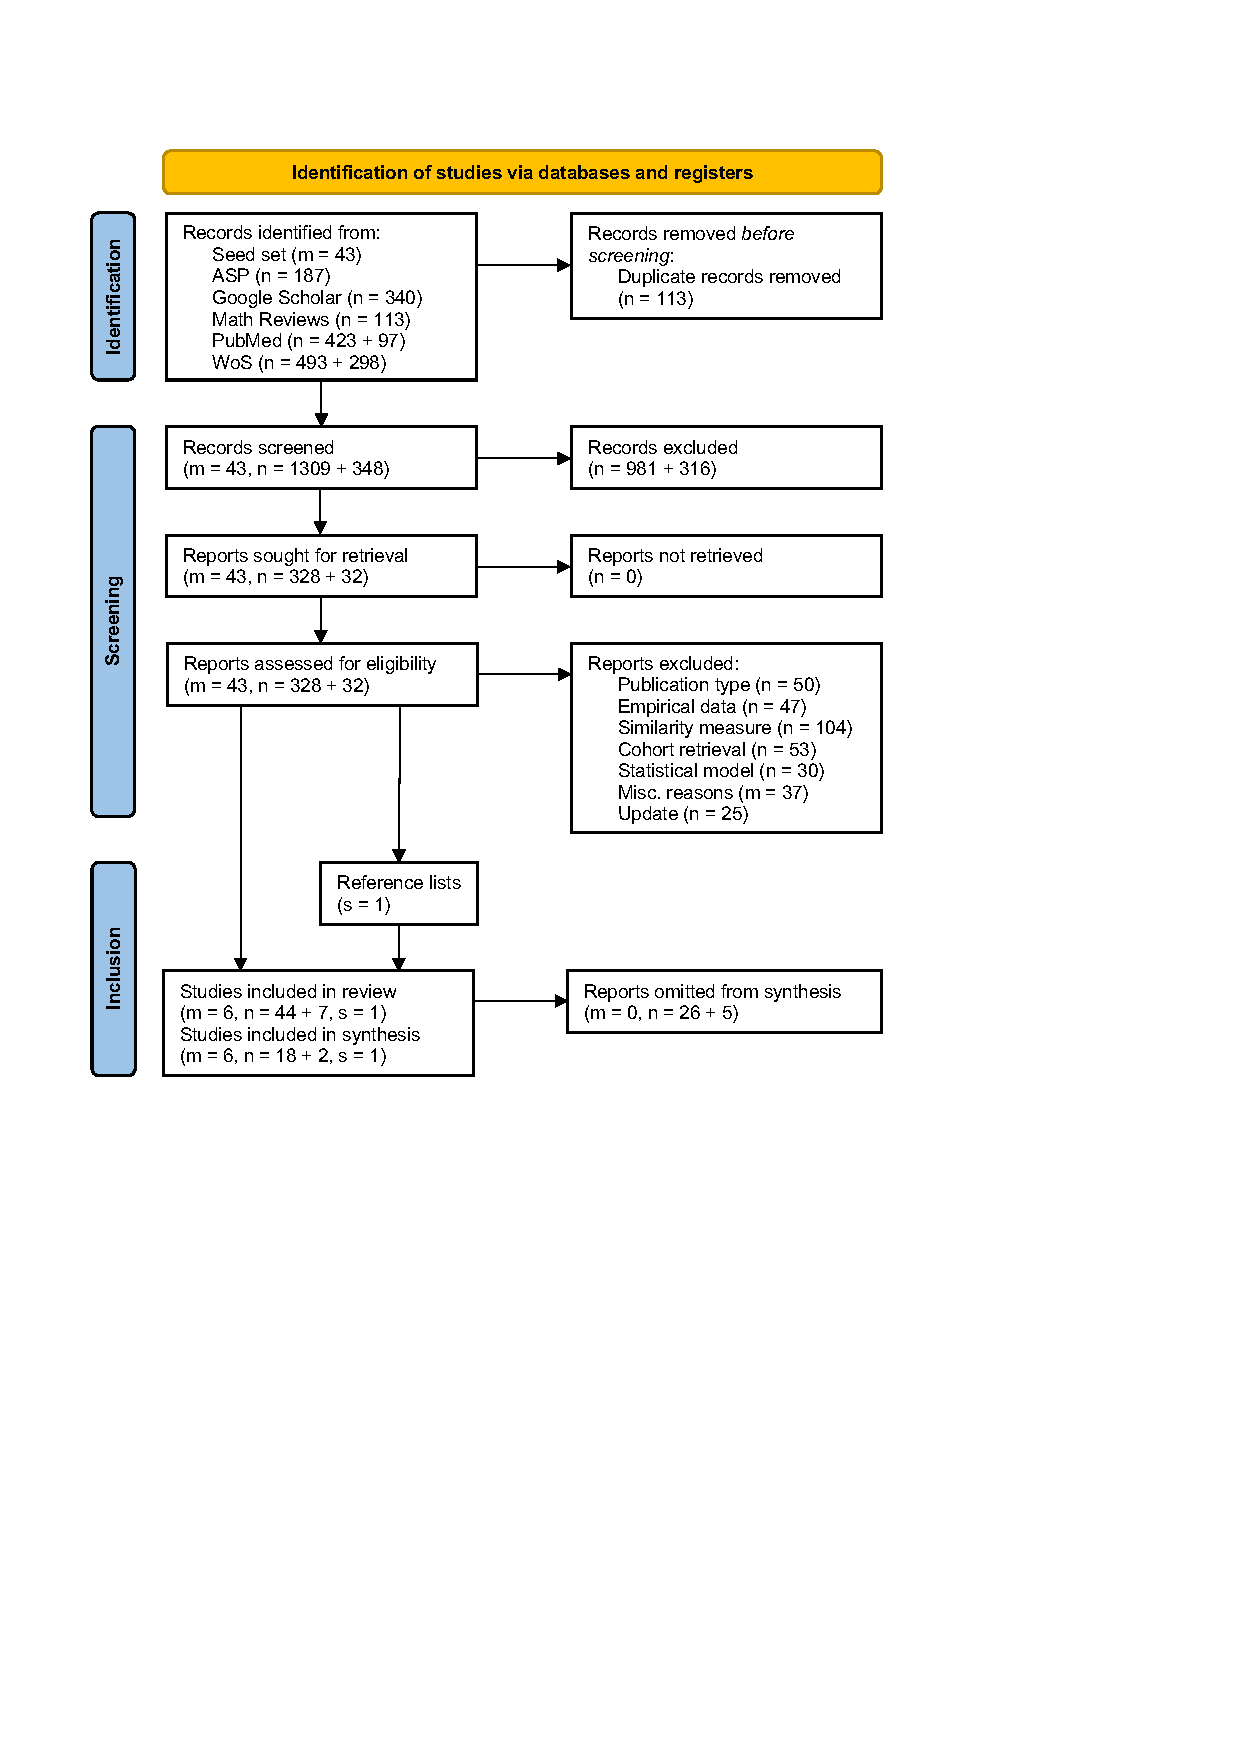
\includegraphics[width=0.8\linewidth]{Fig1} 

}

\caption{\hl{PRISMA-S flow chart.}
 Lowercase letters refer to items obtained from
 the seed set (m),
 the structured search (n), and
 citation/reference tracking (s).
 Within the structured search results,
 summands correspond to original and update.}\label{fig:prisma}
\end{figure}

From the first search results, there were 60 disagreements over
inclusion versus exclusion. Inter-rater reliability was low, at 82\%
relative to a 72\% probability of random agreement. Only one author was
available to review full texts from the update search.

We then reviewed \hl{a seed set comprising 43 studies} that inspired
this review. After removing duplicates and screening for eligibility, we
were left with 6 additional studies
\citep{Park2006, Lowsky2013, Lee2015, Ng2015, Lee2017, Wang2019}, 1 of
which was excluded from the synthesis for using \hl{kNN} prediction.
Reference tracking from the 43 + 360 = 403 studies assessed for
eligibility led us to identify 1 additional study that met our criteria
\citep{Kasabov2010}. This left us with 21 + 1 + 5 = 27 studies included
in the review and synthesis.

\subsection{Bibliographic and methodological
properties}\label{bibliographic-and-methodological-properties}

The 27 included studies were analyzed based on several characteristics,
and we report and describe some observations here (Table
\ref{tab:synthesis}). The studies were published in a variety of
journals, with some of greater frequency, though no single journal
published more than 3. The journal \emph{Evolving Systems} published 2
of the included studies, \emph{Artificial Intelligence in Medicine}
published 3, \emph{Hindawi - Journal of Healthcare Engineering}
published 3, \emph{Evolving Systems} published 2, and \emph{PLOS One}
published 2.

Another interesting pattern lay in the years of publication (Figure
\ref{fig:year}). While these studies trace back to the late 1990s, they
have become \hl{slightly }more common, which suggests that this is an
active, though not rapidly expanding, approach. We note that CBR in
health and medicine originated as early as 1990, and \hl{SCBM} emerged
soon after CBR had established itself; the idea has been ``in the air''
for as long as CBR has been in use.
\hl{ Based on the motivations and methodologies observed in our sample (discussed in later sections), we speculate that the higher frequency of studies since 2013 is attributable in large part to the availability of vaster clinical databases with improved pre-processing tools, following the rapid uptake of EHRs; and of more efficient and powerful tools for retrieval (similarity-matching), the traditional bottleneck of CBR. Another possibility is an increased interest in interpretable machine learning }\citep{Rudin2022}\hl{. Each of these factors should apply with no less force to other CDSS and clinical applications of ML, and the rise we see may simply be commensurate with an overall increase in the volume of articles in these fields.}

\small

\begin{longtable}[]{@{}
  >{\raggedright\arraybackslash}p{(\columnwidth - 12\tabcolsep) * \real{0.1123}}
  >{\raggedright\arraybackslash}p{(\columnwidth - 12\tabcolsep) * \real{0.1497}}
  >{\raggedright\arraybackslash}p{(\columnwidth - 12\tabcolsep) * \real{0.1176}}
  >{\raggedright\arraybackslash}p{(\columnwidth - 12\tabcolsep) * \real{0.1925}}
  >{\raggedright\arraybackslash}p{(\columnwidth - 12\tabcolsep) * \real{0.1497}}
  >{\raggedleft\arraybackslash}p{(\columnwidth - 12\tabcolsep) * \real{0.1283}}
  >{\raggedleft\arraybackslash}p{(\columnwidth - 12\tabcolsep) * \real{0.1497}}@{}}
\caption{\label{tab:synthesis}\hl{Studies included in the method synthesis, arranged by the earliest the study is known to have been public.}}\tabularnewline
\toprule\noalign{}
\begin{minipage}[b]{\linewidth}\raggedright
Citation
\end{minipage} & \begin{minipage}[b]{\linewidth}\raggedright
Task
\end{minipage} & \begin{minipage}[b]{\linewidth}\raggedright
Aim
\end{minipage} & \begin{minipage}[b]{\linewidth}\raggedright
Source
\end{minipage} & \begin{minipage}[b]{\linewidth}\raggedright
Type
\end{minipage} & \begin{minipage}[b]{\linewidth}\raggedleft
Cases
\end{minipage} & \begin{minipage}[b]{\linewidth}\raggedleft
Features
\end{minipage} \\
\midrule\noalign{}
\endfirsthead
\toprule\noalign{}
\begin{minipage}[b]{\linewidth}\raggedright
Citation
\end{minipage} & \begin{minipage}[b]{\linewidth}\raggedright
Task
\end{minipage} & \begin{minipage}[b]{\linewidth}\raggedright
Aim
\end{minipage} & \begin{minipage}[b]{\linewidth}\raggedright
Source
\end{minipage} & \begin{minipage}[b]{\linewidth}\raggedright
Type
\end{minipage} & \begin{minipage}[b]{\linewidth}\raggedleft
Cases
\end{minipage} & \begin{minipage}[b]{\linewidth}\raggedleft
Features
\end{minipage} \\
\midrule\noalign{}
\endhead
\bottomrule\noalign{}
\endlastfoot
\citet{Yearwood1997} & Recommend-ation\hspace{6em} &
Practice\hspace{6em} & Clinical\hspace{6em} &
Cross-sectional\hspace{6em} & 1,355 & 9 \\
\citet{Mariuzzi1997} & Prognosis\hspace{6em} & Knowledge\hspace{6em} &
Clinical\hspace{6em} & Longitudinal\hspace{6em} & 113 & 4 \\
\citet{Wyns2004} & Diagnosis\hspace{6em} & Practice\hspace{6em} &
Laboratory\hspace{6em} & Cross-sectional\hspace{6em} & 160 & 14 \\
\citet{Park2006} & Diagnosis\hspace{6em} & Practice\hspace{6em} &
Clinical, Imaging\hspace{6em} & Cross-sectional\hspace{6em} & 366; 270;
560; 760; 340 & 35; 14; 31; 8; 7 \\
\citet{Song2006} & Prognosis\hspace{6em} & Practice\hspace{6em} &
Clinical\hspace{6em} & Cross-sectional\hspace{6em} & 1,000 & 6 \\
\citet{Elter2007} & Diagnosis\hspace{6em} & Practice\hspace{6em} &
Clinical\hspace{6em} & Cross-sectional\hspace{6em} & 2,620 & 6 \\
\citet{Xu2008} & Prognosis\hspace{6em} & Practice\hspace{6em} &
Clinical\hspace{6em} & Cross-sectional\hspace{6em} & 67 & 14 \\
\citet{Lopez2011} & Diagnosis\hspace{6em} & Knowledge\hspace{6em} &
Clinical\hspace{6em} & Cross-sectional\hspace{6em} & 871 & 4 \\
\citet{Kasabov2010} & Diagnosis\hspace{6em} & Knowledge\hspace{6em} &
Clinical\hspace{6em} & Cross-sectional\hspace{6em} & 62 & 2,000 \\
\citet{Verma2015} & Prognosis\hspace{6em} & Practice\hspace{6em} &
Clinical\hspace{6em} & Cross-sectional\hspace{6em} & 74 & 93 \\
\citet{Liang2015} & Diagnosis\hspace{6em} & Practice\hspace{6em} &
Clinical\hspace{6em} & Cross-sectional\hspace{6em} & 62; 72; 77; 181 &
2,000; 7,129; 7,129; 12,533 \\
\citet{Lowsky2013} & Prognosis\hspace{6em} & Practice\hspace{6em} &
Clinical, Laboratory\hspace{6em} & Longitudinal\hspace{6em} & 13,525 &
13 \\
\citet{CampilloGimenez2013} & Recommend-ation\hspace{6em} &
Practice\hspace{6em} & Patient-reported\hspace{6em} &
Cross-sectional\hspace{6em} & 1,647 & 18 \\
\citet{Nicolas2014} & Diagnosis\hspace{6em} & Knowledge\hspace{6em} &
Clinical\hspace{6em} & Cross-sectional\hspace{6em} & 150 & 83 \\
\citet{Ng2015} & Prognosis\hspace{6em} & Practice\hspace{6em} &
Clinical, Laboratory\hspace{6em} & Longitudinal\hspace{6em} & 7,519 &
130 \\
\citet{Lee2015} & Prognosis\hspace{6em} & Knowledge\hspace{6em} &
Clinical, Laboratory\hspace{6em} & Cross-sectional\hspace{6em} & 17,152
& 75 \\
\citet{Vilhena2016} & Diagnosis\hspace{6em} & Knowledge\hspace{6em} &
Clinical\hspace{6em} & Cross-sectional\hspace{6em} & 1,046 & 8 \\
\citet{Lee2017} & Prognosis\hspace{6em} & Practice\hspace{6em} &
Clinical, Laboratory\hspace{6em} & Cross-sectional\hspace{6em} & 17,152
& 75 \\
\citet{Zhang2018} & Diagnosis\hspace{6em} & Knowledge\hspace{6em} &
Imaging\hspace{6em} & Cross-sectional\hspace{6em} & 302 & 8 \\
\citet{Malykh2018} & Recommend-ation\hspace{6em} & Practice\hspace{6em}
& Clinical\hspace{6em} & Cross-sectional\hspace{6em} & 638 & 49,728 \\
\citet{Ma2020} & Prognosis\hspace{6em} & Practice\hspace{6em} &
Clinical\hspace{6em} & Cross-sectional\hspace{6em} & 4,000 & 22 \\
\citet{Wang2019} & Diagnosis\hspace{6em} & Practice\hspace{6em} &
Clinical, Laboratory\hspace{6em} & Cross-sectional\hspace{6em} & 16,490
& 106 \\
\citet{Wang2020} & Recommend-ation\hspace{6em} & Practice\hspace{6em} &
Clinical\hspace{6em} & Cross-sectional\hspace{6em} & 8 & 5 \\
\citet{Tang2021}; \citet{Ng2021} & Recommend-ation\hspace{6em} &
Practice\hspace{6em} & Clinical\hspace{6em} & Longitudinal\hspace{6em} &
245,825 & 1,466,474 \\
\citet{Liu2022} & Prognosis\hspace{6em} & Knowledge\hspace{6em} &
Clinical, Laboratory\hspace{6em} & Cross-sectional\hspace{6em} & 76,597
& 1,892 \\
\citet{Doborjeh2022} & Prognosis\hspace{6em} & Practice\hspace{6em} &
Clinical, Environmental\hspace{6em} & Longitudinal\hspace{6em} & 804 &
46 \\
\end{longtable}

\normalsize

\begin{figure}

{\centering 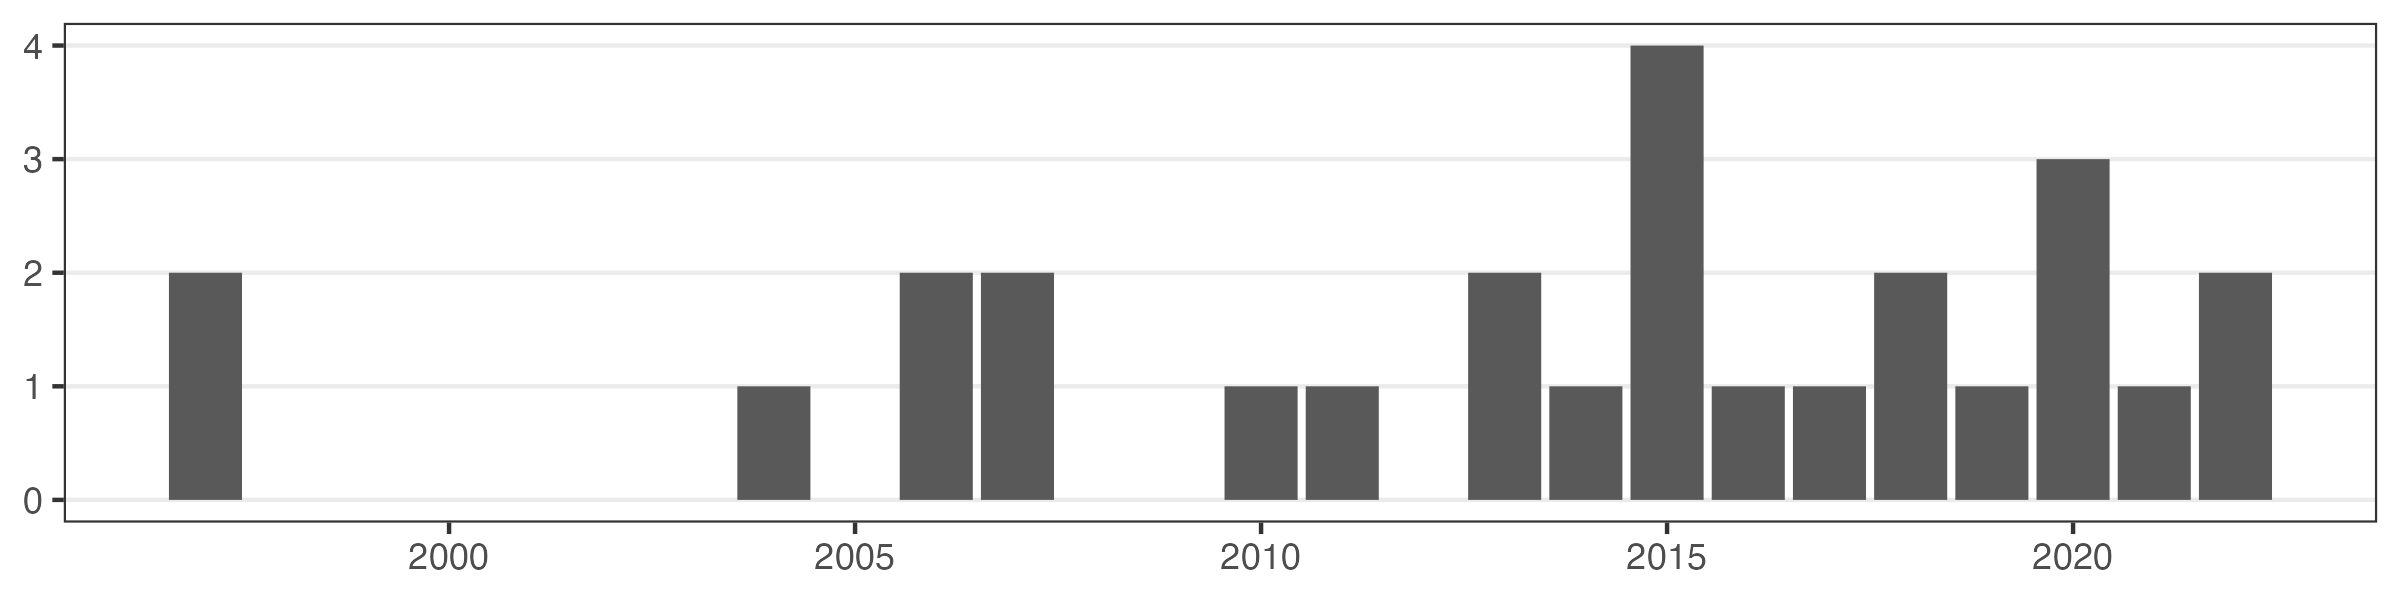
\includegraphics[width=1\linewidth]{Fig2} 

}

\caption{Number of publications in our sample each year.}\label{fig:year}
\end{figure}

Another dominant characteristic of included studies is their broader
remit. We categorized studies as ``knowledge'' or ``practice'' based on
whether their aim was to produce generalizable knowledge or to improve
practice. We classified 8 of the studies as ``knowledge'', making the
majority of studies from a ``practice'' standpoint. These studies aimed
to provide tools for use in clinic or to improve outcomes.

\hl{Most studies used clinical data elements alone
(16),
and most of the remainder used these in combination with laboratory
(6),
imaging
(1),
or environmental
(1)
data. The data source was related to the modeling task, for instance in that all decision support models used either clinical or patient-reported data.
The mosaic plot in Figure }\ref{fig:properties}\hl{ summarizes the relation between data source, clinical task, and aim.}

Lastly, we observed a commonality among 6 of the included studies in
having evaluated methods using leave-one-out cross-validation (LOOCV).
The purpose of this measure is to estimate the overall performance of
certain factors when used to make predictions, particularly utilized on
smaller data sets, where models benefit greatly from larger training
sets and additional model fitting is less costly.

In addition to the aim of its analysis, we coded several aspects of the
design of each study, including the source and type of data and the
clinical task the model performed (Table \ref{tab:synthesis}), as well
as the specific methodology and terminology adopted (Table
\ref{tab:composite}). In the following subsections, we take a closer
look at these design elements and their reported justifications and
limitations.

\subsection{Application domains}\label{application-domains}

While all included studies were reported in scientific and medical
journals, the vast majority were oriented toward clinical practice
rather than medical research. For example, a 2006 study specifically
evaluated the usefulness of CBR-based explanations for the purpose of
decision support \citep{Doyle2006}. This study was part of a much larger
literature on CBR systems and was included here despite relying on
\hl{kNN} prediction because it used an unconventional voting scheme to
generate recommendations. A more recent study took essentially the same
focus with respect to a proposed clinical risk prediction model, which
amounted to CBR with a novel weighting scheme on predictors informed by
expert consensus \citep{Fang2021}. In both cases a prototype
implementation was \hl{evaluated} in an experimental \hl{setting.}

The most common clinical motivations were individualized detection or
diagnosis, prognosis or outcome prediction, and treatment or care
recommendation. The plurality focused on prognosis or outcome
prediction, often using time-to-event analysis: \citet{Mariuzzi1997}
used CBR to predict survival time from several geometric properties of
breast tumors. \citet{Lowsky2013} used CBR with non-parametric survival
models on registry data to predict patient--graft survival times
following kidney transplantation. \citet{Lee2015} and \citet{Lee2017}
used localized \hl{GLM} and RF modeling to predict 30-day mortality
following discharge for ICU patients. \citet{Vilhena2016} developed a
CBR cycle around a clustering-informed similarity matching procedure and
an \hl{ANN}--based classifier to identify thrombophilia patients at high
risk of thrombotic episodes. \citet{Ma2020} took a similarity
cohort--based approach to predicting length of stay for ICU patients.
\citet{Doborjeh2022} localized spiking \hl{ANN}s in order to assess
stroke risk from up to 7-day time series of clinical and environmental
factors. \citet{Liu2022} incorporated global-to-local transfer learning
into \hl{SCBM}s of acute kidney injury risk in hospitalized patients.
Also of note, from a public health perspective, \citet{Xu2008} used CBR
to predict rehabilitation time as well as disability risk for unemployed
workers experiencing chronic pain.

Toward detection and diagnosis, \citet{Wyns2004} proposed a hybrid
neural net--CBR system to distinguish (with confidence bounds) arthritic
versus control patients, based on several histological features.
\citet{Nicolas2014} used collaborative multilabel CBR to subtype
melanoma patients based on confocal and dermoscopy images.
\citet{Wang2019} used \hl{SCBM}s built from a multi-type additive
similarity measure to distinguish type 2 diabetic versus control
populations. Along the way, \citet{Song2006}, \citet{Kasabov2010}, and
\citet{Verma2015} took an iterative model-building approach to several
tasks: predicting glomerular filtration rate, a key indicator of renal
function, from demographic and physiological variables; identifying
patients with colon cancer using a large number of gene expression
measurements; and identifying patients with type 2 diabetes based on
demographic, physiological, and genetic variables.

While several studies emphasized the potential or actual value to
decision-making of their methods and tools, only one incorporated
treatment decisions into their approach: By taking ``decision points''
as their units of analysis, \citet{Tang2021} and \citet{Ng2021} built
not classifiers or predictors but comparative effectiveness models into
a localized framework, providing for the first time in our sample
explicitly prescriptive rather than descriptive clinical decision
support.

A partial exception to this focus was a 2014 study that also reported a
decision support tool, in this case for early diagnosis of melanoma from
clinical data and dermoscopy images \citep{Nicolas2014}. While the
stated objectives were analogous, specific emphasis was placed on the
acquisition of new knowledge through the development of the tool,
including the systematic generation of new data and creation of a
clinical ontology. This study was included for its use of a
collaborative classifier that drew from multiple modeling approaches. In
keeping with this focus of the included literature, the stated
objectives of the proposed methods were more often (or additionally) to
predict outcomes or to recommend interventions than only to diagnose
disease.

\begin{figure}

{\centering 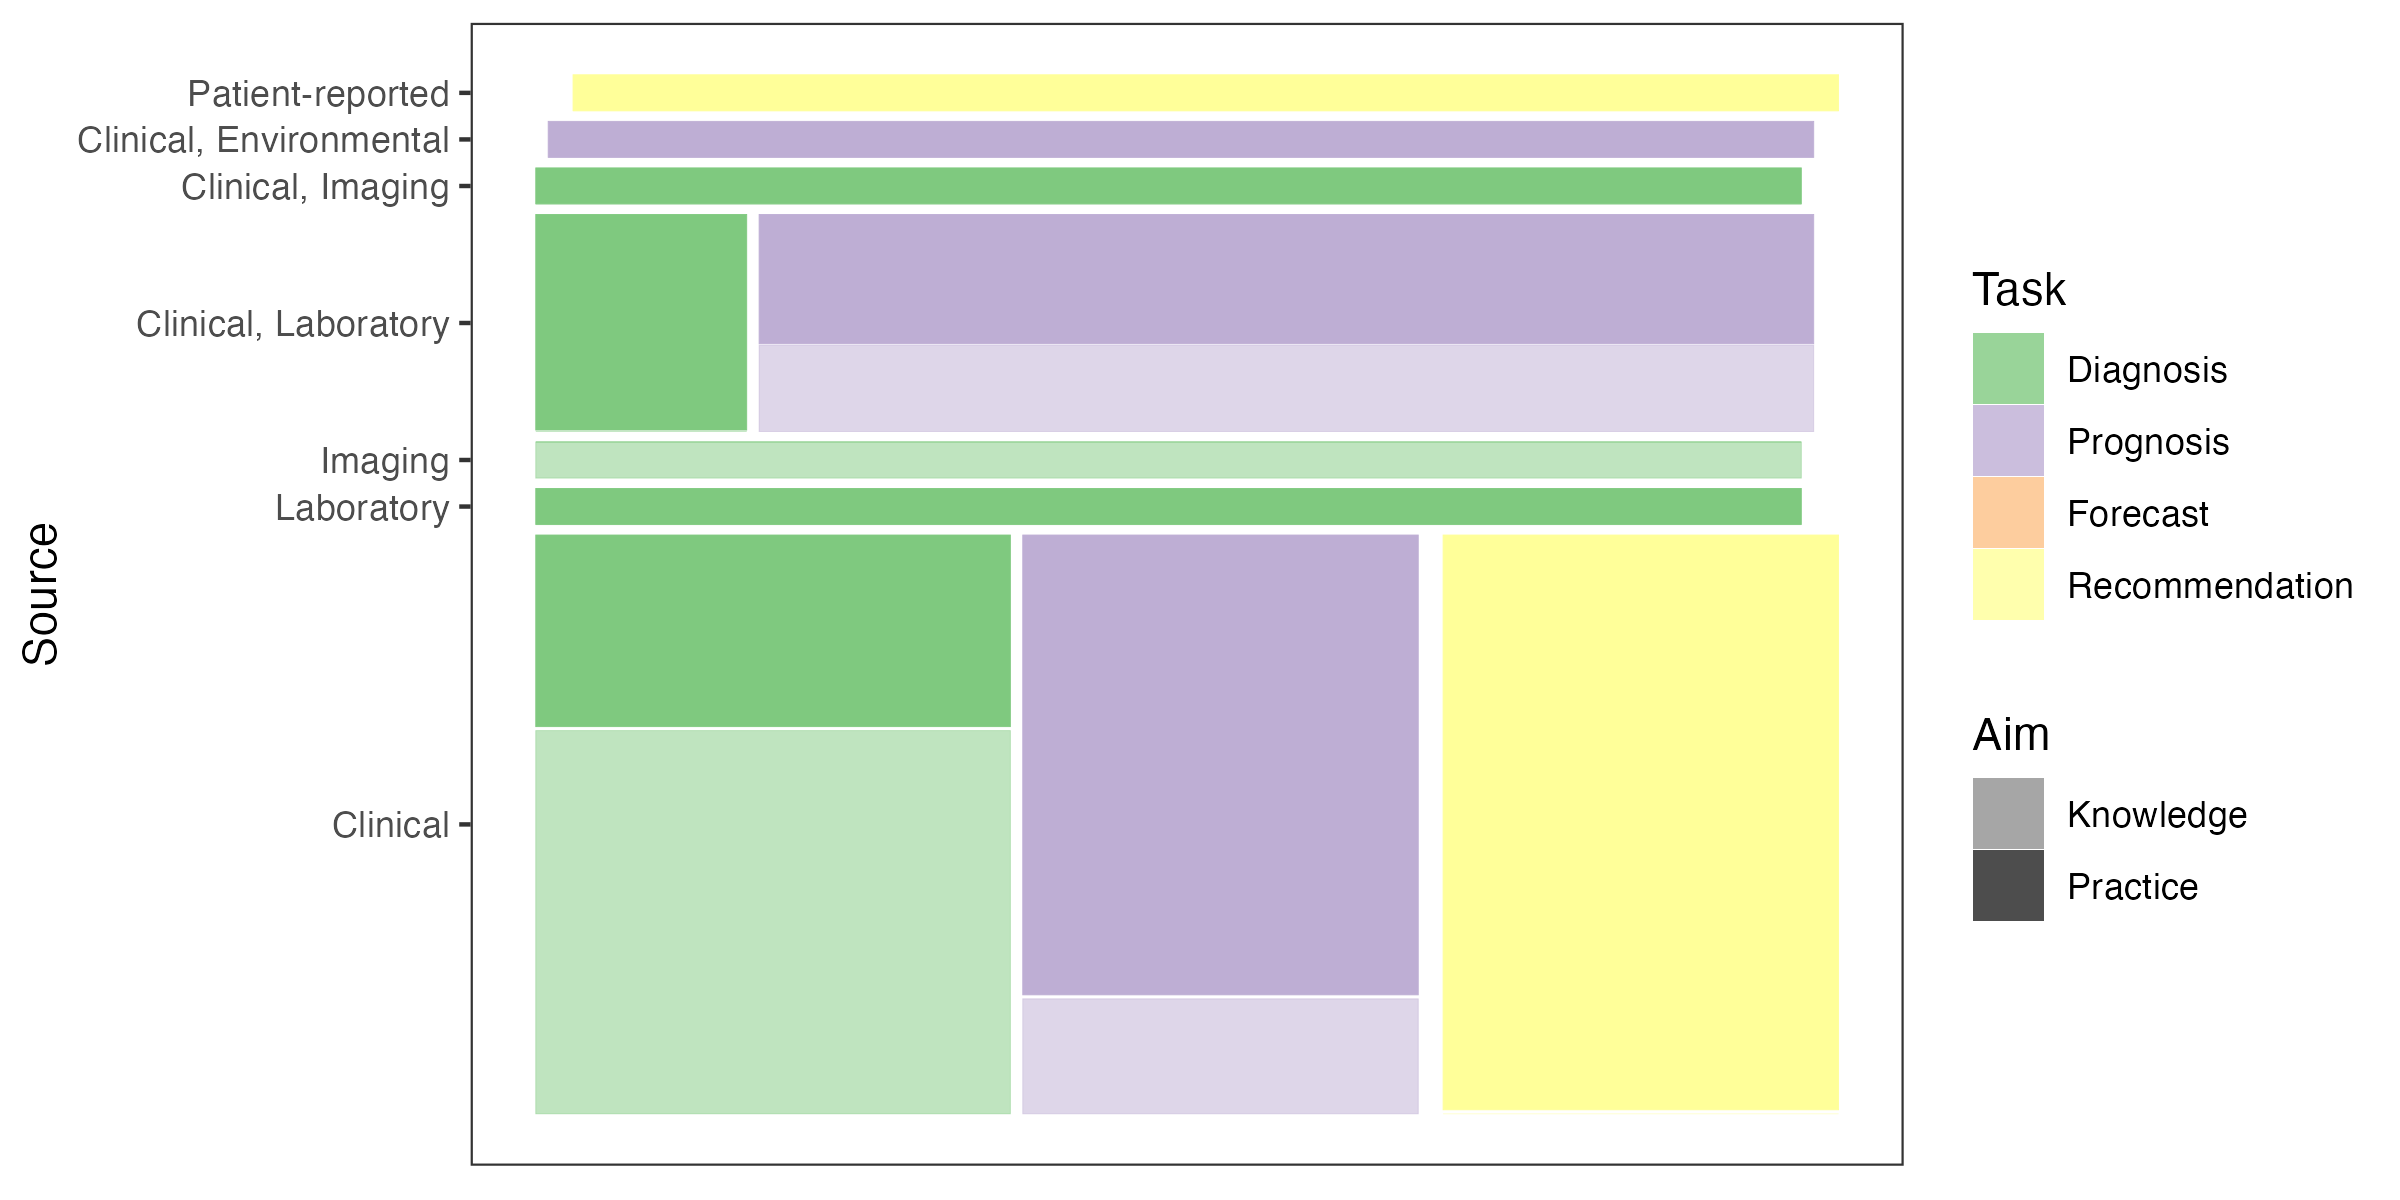
\includegraphics[width=1\linewidth]{Fig3} 

}

\caption{\hl{Share of studies characterized by several design elements:}
 data source (row),
 clinical task (fill), and
 remit (opacity).}\label{fig:properties}
\end{figure}

\subsection{\texorpdfstring{Challenges\hl{ faced}}{Challenges}}\label{challenges}

CBR can be understood as the opposite side of a trade-off with
rule-based reasoning between model size and model complexity:
\citet{Doyle2006} describe their approach as ``knowledge-light'', in
that ``the cases do not contain explicit explanation structures;
instead, explanation is achieved by comparison of the query case with
retrieved cases''. This means that the greatest performance and
efficiency challenges in CBR have to do with the retrieval and revision
phases in the R4 cycle. Several studies addressed these challenges:
\citet{Park2006}, while excluded from the synthesis, were the earliest
to propose that cohorts be bounded by a similarity threshold rather than
by the number of cases, which improved performance in their experiments.
\citet{CampilloGimenez2013} leveraged predictor weights obtained from
logistic regression to inform the similarity calculation used in
retrieval. \citet{Lowsky2013} used non-parametric models to reduce the
computational burden of revision (prediction). \citet{Ma2020} proposed
to improve efficiency along the entire R4 cycle, but in particular by
only executing task-dependent steps in real time (``just-in-time
learning'', JITL), and \citet{Ng2021} and \citet{Tang2021} partitioned
multiple phases in the R4 cycle into offline and online components, only
the latter of which would be performed in real time as new data are
received. \citet{Liu2022} used transfer learning from globally-fitted
models to improve the efficiency of \hl{SCBM}s.

Other studies addressed limitations of available tools.
\citet{Lopez2011} implemented a comprehensive CBR tool in response to
the lack of general-purpose software, to enable coupling with other
tools as well as to expedite development, experimentation, and uptake.
Several other teams also set out to develop more generalizable and
data-agnostic clinical support tools
\citep{Elter2007, Liang2015, Ng2015, Zhang2018}. However, more
informatical and legal challenges to implementation, including
interoperability of systems and data and regulations concerning security
and privacy, were rarely addressed. We discuss this further in Section
\ref{future-work}.

Figure \ref{fig:methods} compares the rates at which several
methodological elements are invoked in the sample.

\subsection{Evaluations}\label{evaluations}

Most included studies quantitatively compared the predictive performance
of their proposed method(s) to one or more comparators. What we took to
be the signature results are collated in Table \ref{tab:performance} in
the Appendix. Note that we exercised some judgment in classifying
methods as proposals and comparators, as in some cases all methods were
original but only some showcased main ideas. It would be impractical to
meta-analyze these numbers due to the great variety of settings,
problems, data types, techniques, and choices involved.

We do observe one clear pattern: All of the proposed methods that most
evidently outperformed their comparators---Kohonen + CBR
\citep{Wyns2004}, TWNFI \citep{Song2006, Kasabov2010}, gravitational
search algorithms (GSA) \citep{Liang2015}, CBR + rules (+ DML)
\citep{Nicolas2014}, Gaussian process regression \citep{Zhang2018},
JITL-ELM \citep{Ma2020}---are hybrids of \hl{SCBM} (in some cases CBR)
with other techniques, often DML. Though \citet{CampilloGimenez2013} and
\citet{Ng2015} report non-superior performance by such hybrids, the
pattern suggests the importance of the similarity measure to the
retrieval step. Meanwhile, when proposed approaches targeted cohort
demarcation or choice of predictive model---statistical CBR
\citep{Park2006}; individualized \hl{GLM, DT, and RF}
\citep{Lee2015, Lee2017}---they did not consistently outperform
comparators.

\hl{Figure }\ref{fig:performance}\hl{ visualizes the relationship between performance and case count, feature count, data source, and predictive task for those experiments that evaluated models using accuracy or AUROC (other performance measures were too rare to allow for useful comparisons).
While not represented in the plot, results from different models applied to the same data can be inferred from their common case counts, data sources, and tasks.
The data are too heterogeneous to meaningfully test for trends. Performance varies much more between experiments than between models within experiments, and there is no clear dependency on the source(s) of data or on the type of prediction.
We also note that the plot is no less consistent with the alarming negative association between sample size and reported accuracy observed by }\citet{Berisha2021}\hl{ than with the inverse association expected in the absence of selective reporting.}

\subsection{Identified needs}\label{identified-needs}

\hl{S}tudy authors focused their recommendations and \hl{future plans}
mostly on technical improvements and evaluations\hl{.} Urged
improvements included full or partial automation of predictor selection
\citep{Mariuzzi1997, Yearwood1997}, similarity learning
\citep{Mariuzzi1997, Wang2019}, and parameter optimization
\citep{Song2006, Lee2017}; extensions to new data structures
\citep{Lopez2011}, data types \citep{Liang2015, Verma2015, Malykh2018},
and reasoning systems \citep{Nicolas2014}; and the use of more advanced
model components to improve accuracy or efficiency
\citep{Lowsky2013, Lee2015, Liang2015, Zhang2018}. Authors also urged
validations and independent evaluations using larger or more
comprehensive data sets \citep{Elter2007, Xu2008, Verma2015, Ng2015},
using data aggregated from multiple health systems
\citep{Lee2015, Lee2017, Tang2021, Ng2021}, and in other care settings
or disease contexts \citep{Song2006, Zhang2018, Tang2021, Ng2021}.
\hl{That said, s}ome authors urged the incorporation of (human-derived)
domain knowledge into the data or models
\citep{Yearwood1997, Wang2019}\hl{, and o}thers suggested new uses of
their \hl{methods} to measure feature importance \citep{Wyns2004}, to
make models more expressive \citep{Lee2015}, and to combine information
obtained both from global and from \hl{SCBM}s \citep{Ng2015}. \hl{(}Most
of this incremental work was indeed carried out \hl{later} in our
sample.\hl{)}

\section{\texorpdfstring{\hl{Discussion}}{}}\label{section}

After commenting briefly on our review process, we draw several
observations from our encoding of the included studies. We first focus
on their methodological choices and innovations, then on their
conventions and language. We spend most of the section discussing the
differences and commonalities of the techniques used, toward a general
method that encompasses most or all cases. We then suggest some avenues
for future studies and conclude with our key takeaways.

\subsection{Process}\label{process}

The low inter-rater reliability was due, in parts, to different
interpretations of some eligibility criteria by the authors,
inconsistent terminology across the sample, and incomplete reporting of
resources and methods in the sample. Regarding interpretation of
criteria, some wording of the criteria was adjusted following
discussions between the reviewing authors during full-text review to
better specify an agreed-upon meaning. \hl{We }discuss the different
domains, terminologies, and reporting issues of the sample in the
remainder of this section.

\subsection{Study designs}\label{study-designs}

Consistent with their orientation, almost all included studies were
conducted using clinical data, only occasionally together with
patient-reported (2), laboratory (3), image (1), and environmental (1)
data. We suggest three reasons for this: First, this literature traces
back to the 1990s, before -omic data could be generated cost-effectively
at scale. Second, CBR in particular has a strong tradition in clinical
decision support, where the focus of our sample remains throughout the
review period. Third, because most -omic data are highly
homogeneous---all measurements are made along or can be transformed to a
common scale, e.g.~greyscale pixellations for X-ray images and
transcripts per million for RNA-seq data---more deeply theoretical
analysis techniques have been developed and come into wide use. While
variations on correlation-based approaches like EHR-based phenome-wide
association studies and similarity-based methods like CBR itself have
been developed, more mechanistic and probabilistic tools have not become
a domain standard.

\subsection{Coherence}\label{coherence}

The motivational and methodological unity of these studies does not
reflect a unified research program. Besides the lack of any primary
journal of record, we observed collaborations only among the authors of
smaller contiguous programs, including applications of the TWNFI
methodology \citep{Song2006, Verma2015}, individualized mortality
prediction for ICU patients \citep{Lee2015, Lee2017} and the use of more
explanatory models to prioritize predictors or treatments for chronic
disease \citep{Ng2015, Tang2021, Ng2021}.

\subsection{Synthesis}\label{synthesis-1}

The 27 studies included in our synthesis used composite techniques that
we organized into two major types. One type, \emph{similarity learning},
was used in 8 studies that tie in to the much larger literature on DML
\citep{Yang2006}. The other, \emph{cohort thresholding}, focused on
choosing or optimizing the manner in which cohorts were demarcated using
the similarity measure.

\subsubsection{Similarity learning and threshold
optimization}\label{similarity-learning-and-threshold-optimization}

\hl{Eight} studies used response values in training data sets to
supervise similarity learning while two used unsupervised learning
(Table \ref{tab:composite}). Based on the key properties of DML
algorithms identified by \citet{Bellet2014}, most learned measures were
non-linear while some were locally learned, and some were optimized
globally while others locally. Not all qualified as DML, since the
resulting measures would not necessarily satisfy the triangle
inequality. Each used its similarity measure to retrieve training cases
relevant to each testing case. \hl{Most} took a standard \hl{kNN}
approach to generating predictions; \hl{two}
\citep{Vilhena2016, Tang2021} fit predictive models to the retrieved
cohorts.

Several studies used unsupervised similarity learning, for example the
Mahalanobis distance \citep{Lowsky2013} and the Kolmogorov entropy-based
distance \citep{Elter2007}. In particular, \citet{Yearwood1997} defined
similarity as a weighted sum of differences in predictor values and used
linear regression to optimize the weights for the predictive accuracy of
the cohort they retrieve. Others used supervised learning:
\citet{Song2006} proposed an iterative algorithm to optimize a set of
fuzzy inference rules used to retrieve relevant cases and generate a
prediction, using back-propagation on the rules' parameters. Their
method was used in several later studies returned by our search, which
are not discussed here because they did not originate the technique.
\citet{Nicolas2014} explicitly appeal to a supervised distance metric
learning (DML) technique \citep{Xing2002} to obtain a similarity measure
on their set of dermoscopy and confocal images that most effectively
separates malignant from benign melanoma tumors. We will discuss the
remaining uses of supervised similarity learning shortly.

Distinct from but related to similarity learning was supervised cohort
construction. This was an adaptive step taken by \citet{Park2006} to
optimize the predictive performance of models fitted to cohorts
retrieved using a fixed similarity rather than count threshold, a
counterpart to conventional CBR they called ``statistical
CBR''.\footnote{Drawing from \citet{Goyal2008}, we suggest the term
  ``combinatorial CBR'' for the then-conventional approach using
  similarity cohorts of fixed cardinality.} The step used a heuristic
procedure to locate a similarity threshold that (locally) maximizes
predictive accuracy on the training set. This is analogous to optimizing
the neighborhood size parameter in \hl{kNN} predictive modeling, so we
will not discuss it further except to mention that the authors found
statistical CBR to outperform conventional CBR on several data sets.
\citet{CampilloGimenez2013} combined these learning techniques: They
used logistic regression on the training set to obtain weights for the
predictors (by predicting the binary outcome of kidney transplant
waitlist registration) and for the cases (by predicting agreement of
outcome between an index case and other training cases), and they used
exhaustion to optimize the size of the retrieved cohort for the accuracy
of the \hl{kNN} model using the previously optimized weights.

\subsubsection{Localized models}\label{localized-models}

\hl{Seven} other studies employed localized models:
\citet{Mariuzzi1997}, \citet{Lee2015}, \citet{Verma2015},
\citet{Wang2019}, \citet{Ma2020}, \citet{Liu2022}, and
\citet{Doborjeh2022}. \hl{Most} models were purely
predictive\hl{, though} \citet{Mariuzzi1997} produced purely descriptive
models of survival outcomes, which were evaluated for their precision
rather than their accuracy, while \citet{Ng2015} used generalized
regression models descriptively as well as predictively, as did
\citet{Tang2021}, \citet{Ng2021}, and \citet{Liu2022}\hl{.} The most
common approach to cohort selection was to optimize a size threshold via
manual exploration
\citep{Mariuzzi1997, Lee2015, Ng2015, Lee2017, Wang2019, Vilhena2016} or
via cross-validation \citep{Lowsky2013, Verma2015}. \hl{One} study
\citep{Ma2020} set a fixed cohort size while two
\citep{Liang2015, Tang2021, Ng2021} devised more sophisticated
algorithms to balance multiple desiderata including predictive accuracy.

\hl{One theme} was the optimization of retrieved cohort sizes for some
measure of model performance. Despite the early recommendation by
\citet{Park2006} to threshold cohorts by similarity rather than by
cardinality, only the one previously published study
\citep{Mariuzzi1997} and the most recent study \citep{Tang2021, Ng2021}
in this corpus took this approach, though \citet{Liu2022} took a third
option by retrieving fixed proportions of training data. Viewed as a
hyperparameter of the individualized modeling approach, cohort size can
be treated in the same way as neighborhood size in \hl{kNN}
\hl{prediction}, so we will not discuss it further.

\citet{Kasabov2010} proposed an iterative algorithm to settle on an
optimal number and set of predictors as well as number of training cases
(comprising the retrieved cohort) that was later used by
\citet{Liang2015}. More recently, \citet{Tang2021} and \citet{Ng2021}
proposed a three-step process for cohort selection that filtered by
exact match for one subset of predictors, used domain-informed
similarity measures to rank these, and optimized the similarity
threshold for a trade-off between cohort size and a measure of bias
called cohort balance. \hl{T}hough their similarity measure was
supervised, this optimization process was not.

With the exception of the descriptive survival models of
\citet{Mariuzzi1997}, only one thread in this corpus \hl{concerned the}
interpretability of localized models: \citet{Ng2015} fit logistic
regression models to similarity-based cohorts and examined not only
their predictive performance but the localized sets of largest and most
detectable predictors, termed risk profiles, and how they differed
across the testing population. This approach informed their later use of
localized comparative effectiveness--style models to recommend courses
of treatment at decision points during a monitored patent's stay
\citep{Tang2021, Ng2021}, and it was later used by \citet{Liu2022} to
show a dependency of predictor importance on the patient disease
subgroup. These studies suggest \hl{wider} potential for localized
real-world evidence generation, which has long been promoted as a
promise of advances in clinical and health informatics
\citep{Longhurst2014}.

\subsubsection{A general framework}\label{a-general-framework}

This relatively small sample exhibited a wide range of
\hl{designs in both the assembly of pre-processing, retrieval, reuse, and interpretation steps and the specific tools deployed at each}.
Discussion of the \hl{diversity} of \hl{tools} has been summarized above
and published in greater detail in previous reviews
\citep{Choudhury2016, Sharafoddini2017, Parimbelli2018}\hl{. In this section, we focus on the diversity of assemblies. These depend on}
three largely independent choices
\hl{(Figure }\ref{fig:framework}\hl{)}: (1) how to measure the
similarity between cases, (2) how to retrieve a cohort of cases similar
to an index case, and (3) how to generate a prediction or other
statistical insight for the index case from the similarity cohort.

\begin{figure}

{\centering 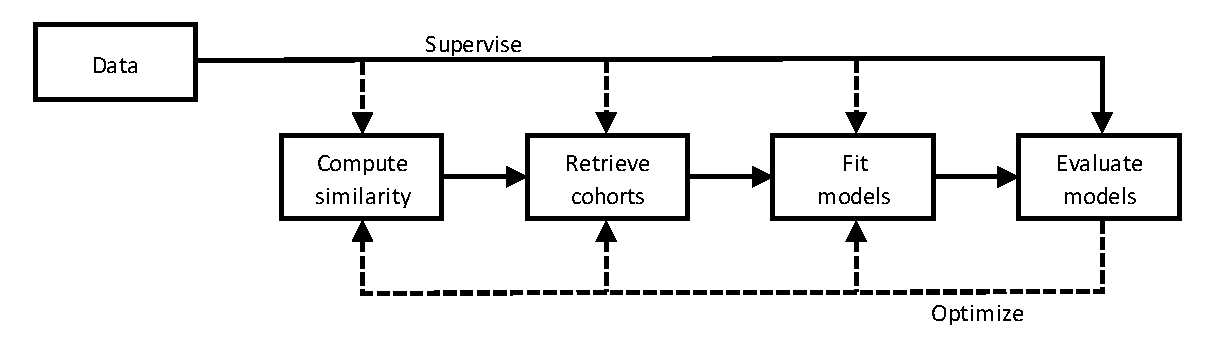
\includegraphics[width=1\linewidth]{Fig5} 

}

\caption{General framework for localized models.
 Dashed arrows indicate optional steps.}\label{fig:framework}
\end{figure}

Each step can be unsupervised supervised: Unsupervised similarity
measures include \hl{the} Levenshtein distance and \hl{cosine}
similarity, while supervised measures include the Mahalanobis distance
and \hl{RF} proximity as well as several composite measures with weights
calculated from the data. Most retrieval steps obtained cohorts with a
uniform size (cardinality) or similarity threshold, and the remaining
were likewise only informed by predictors; thus, while a retrieval step
could in principle be supervised, in this sample none were. Almost all
models were supervised, being that most performed predictive tasks,
though \citet{Mariuzzi1997} modeled only survival rates within localized
cohorts. Meanwhile, each step can be optimized in a ML fashion by having
its parameters tuned to improve performance. We found one study that
tuned the calculation of similarity \citep{Liu2022}, though most uniform
cohort sizes were also tuned. Some earlier studies tuned generalized
regression models, but more recent studies did not.

\hl{As in the case of data and, recently, of ML models, having a standardized general framework facilitates the recombination of ideas and prevents duplicate effort as well as supporting more comprehensive and efficient work [@Ravi2022]. A SCBM implementation based on this framework would help investigators systematically compare predictions and other output obtained using different tools for cohort retrieval and predictive modeling, as well as tune the parameters governing these tools. It would also make like-kind comparisons of performance easier on different tasks using different data sets and expedite validation studies. This would address the core technical needs expressed in our sample (Section }\ref{identified-needs}\hl{) as well as the limitations of our own comparison of reported performances (Section }\ref{evaluations}\hl{).
We also believe that this framework could be used to make the diversity of possible approaches more comprehensible to users, enabling them to most appropriately tailor these decisions to their tasks.}

\small

\begin{longtable}[]{@{}
  >{\raggedright\arraybackslash}p{(\columnwidth - 6\tabcolsep) * \real{0.1928}}
  >{\raggedright\arraybackslash}p{(\columnwidth - 6\tabcolsep) * \real{0.2851}}
  >{\raggedright\arraybackslash}p{(\columnwidth - 6\tabcolsep) * \real{0.1566}}
  >{\raggedright\arraybackslash}p{(\columnwidth - 6\tabcolsep) * \real{0.3655}}@{}}
\caption{\label{tab:framework}Specializations of general framework to
included studies. Flags: R = recurse\hl{d}, S = supervised, T = tuned
(optimized).}\tabularnewline
\toprule\noalign{}
\begin{minipage}[b]{\linewidth}\raggedright
Citation
\end{minipage} & \begin{minipage}[b]{\linewidth}\raggedright
Relevance
\end{minipage} & \begin{minipage}[b]{\linewidth}\raggedright
Retrieval
\end{minipage} & \begin{minipage}[b]{\linewidth}\raggedright
Adaptation
\end{minipage} \\
\midrule\noalign{}
\endfirsthead
\toprule\noalign{}
\begin{minipage}[b]{\linewidth}\raggedright
Citation
\end{minipage} & \begin{minipage}[b]{\linewidth}\raggedright
Relevance
\end{minipage} & \begin{minipage}[b]{\linewidth}\raggedright
Retrieval
\end{minipage} & \begin{minipage}[b]{\linewidth}\raggedright
Adaptation
\end{minipage} \\
\midrule\noalign{}
\endhead
\bottomrule\noalign{}
\endlastfoot
\citet{Mariuzzi1997} & Levenshtein distance\hspace{18em} &
Statistical\hspace{18em} & Survival (S)\hspace{18em} \\
\citet{Yearwood1997} & Weighted sum (S)\hspace{18em} &
Combinatorial\hspace{18em} & Proportion (S)\hspace{18em} \\
\citet{Wyns2004} & Kohonen mapping\hspace{18em} & Adaptive\hspace{18em}
& Representation (S)\hspace{18em} \\
\citet{Park2006} & Euclidean distance\hspace{18em} & Statistical
(T)\hspace{18em} & Weighted sum (S)\hspace{18em} \\
\citet{Elter2007} & Entropic distance\hspace{18em} &
Combinatorial\hspace{18em} & Proportion (S)\hspace{18em} \\
\citet{Xu2008} & Euclidean distance\hspace{18em} &
Combinatorial\hspace{18em} & Proportion (S)\hspace{18em} \\
\citet{Song2006}; \citet{Kasabov2010}; \citet{Liang2015};
\citet{Verma2015} & Feature selection (R,S)\hspace{18em} & Combinatorial
(R)\hspace{18em} & Fuzzy rules (S,T)\hspace{18em} \\
\citet{Lopez2011} & User-defined\hspace{18em} &
User-defined\hspace{18em} & User-defined\hspace{18em} \\
\citet{Lowsky2013} & Mahalanobis distance (S)\hspace{18em} &
Combinatorial (T)\hspace{18em} & Proportional hazards
(S)\hspace{18em} \\
\citet{CampilloGimenez2013} & Weighted overlap\hspace{18em} &
Combinatorial (T)\hspace{18em} & Weighted sum (S)\hspace{18em} \\
\citet{Nicolas2014} & Distance metric learning (S)\hspace{18em} &
Combinatorial\hspace{18em} & Association rules (S,T)\hspace{18em} \\
\citet{Ng2015} & Locally supervised metric learning (S); Feature
selection\hspace{18em} & Combinatorial\hspace{18em} & Logistic model
(S)\hspace{18em} \\
\citet{Lee2015} & Cosine similarity\hspace{18em} & Combinatorial
(T)\hspace{18em} & Logistic model (S); Decision tree (S)\hspace{18em} \\
\citet{Vilhena2016} & Range overlap\hspace{18em} & Clustering
(S)\hspace{18em} & Artificial neural network (S)\hspace{18em} \\
\citet{Lee2017} & Cosine similarity; Random forest proximity
(S)\hspace{18em} & Combinatorial (T)\hspace{18em} & Logistic model (S);
Decision tree (S); Random forest (S)\hspace{18em} \\
\citet{Malykh2018} & Unclear\hspace{18em} & Unclear\hspace{18em} &
Unclear\hspace{18em} \\
\citet{Zhang2018} & Gaussian process model\hspace{18em} &
Complete\hspace{18em} & Weighted support vector machine (S); Weighted
Gaussian process regression (S)\hspace{18em} \\
\citet{Wang2019} & Weighted sum\hspace{18em} & Combinatorial
(T)\hspace{18em} & Logistic model (S); Random forest (S); Nearest
neighbors (S)\hspace{18em} \\
\citet{Ma2020} & Weighted sum\hspace{18em} & Combinatorial\hspace{18em}
& Extreme learning machine (S)\hspace{18em} \\
\citet{Wang2020} & Weighted sum\hspace{18em} & Statistical\hspace{18em}
& Linear model\hspace{18em} \\
\citet{Tang2021}; \citet{Ng2021} & Locally supervised metric learning
(S)\hspace{18em} & Causal inference matching\hspace{18em} & Statistical
test (S)\hspace{18em} \\
\citet{Doborjeh2022} & Euclidean distance; Signal-to-noise ratio
(S)\hspace{18em} & Statistical (T)\hspace{18em} & Spiking neural network
(S)\hspace{18em} \\
\citet{Liu2022} & Weighted Manhattan distance (R,T)\hspace{18em} &
Proportional (T)\hspace{18em} & Logistic model (S)\hspace{18em} \\
\end{longtable}

\normalsize

\subsection{Future work}\label{future-work}

\hl{We suggest four avenues for future work: evaluation of predictive performance, usability and interpretability, practical and regulatory feasibility, and customizability.}

\hl{Most studies were premised on the potential predictive value of localized models (Appendix), but not all experiments affirmed this premise (Section }\ref{evaluations}\hl{). Those that did mostly used DML to improve retrieval and sometimes iteratively optimized the metric and the model.
However, even those that showcased several such specializations }\citep{CampilloGimenez2013, Ng2015, Zhang2018, Liu2022}\hl{ mostly used their own precursors or commonplace alternatives as comparators. Future work should compare competitive alternatives to assess their performance and other trade-offs.
This work would be aided by standardization and modularization using a framework like that outlined above.
For example, }\citet{CampilloGimenez2013}\hl{ and }\citet{Liu2022}\hl{ use a modular design to toggle multiple choices and obtain neatly nested comparisons.}

\hl{While most studies identified outstanding technical needs (Section }\ref{identified-needs}\hl{), few (though some) emphasized the need to assess interpretability, meaningfulness, or trust.
Most studies identified interpretability as an advantage of localized models, though none evaluated model interpretability and few proposed new interpretative uses.
Lack of trust in ML tools is a long-recognized problem that direct intepretability of model components could help alleviate.
One valuable direction for future work would be to measure the utility of interpretable components in research and in clinical practice and the correctness and confidence of users in their interpretations.
Another would be to compare the localized predictor importance measures obtained from localized models to the local importance measures used to explain predictions made by opaque models.}

\hl{Much of the reviewed work was motivated by the need for modeling paradigms that perform well on a variety of tasks and in a variety of settings.
Such software architectures must be robust, versatile, and compliant in the face of diverse data models and use restrictions.
SCBM is susceptible to these challenges, as corpora of past cases must be aggregated from multiple institutions and from multiple systems within institutions, and models built on them must then be applicable to out-of-box data structures.
Individual systems exhibit many dimensions of incompleteness }\citep{Weiskopf2013}\hl{ and vary along other dimensions of quality }\citep{Kohane2021}\hl{, and their aggregation for modeling purposes depends on several kinds of interoperability }\citep{Weber2015}\hl{.
Successful deployment also depends on satisfying regulatory regimes designed to protect the privacy of patients, the security of communications, and trust between parties }\citep{Haendel2021}\hl{.
Future work may therefore eventually need to directly address the challenges of system interoperability and regulatory requirements.}

\hl{From a functionalist approach to reproducibility }\citep{Matarese2022}\hl{, later studies were broadly successful at reproducing earlier studies, and later studies provide sufficient detail to support ongoing reproduction efforts---though these might be limited by the lack of open-source code or public implementations.
However, the immediate goal of most studes was to improve care.
We expect that this practical utility will depend on the ability of the user community to exert control over certain inputs, components, and behaviors of the models.
For one example, a user may want to minimize the weight of rare diseases in medical history in order to retrieve a population with more such cases in order to better measure their associated risk to the outcome. In contrast, they may want to increase the weight of the indicating diagnosis in order to allow fewer patients from similar but distinct populations to influence the model. Alternatively, a user may want to down-weight socioeconomic variables like race--ethnicity in order to ensure a more diverse modeling cohort.
}\citet{Lopez2011}\hl{ took an important step in this direction with an adjustable and adaptable implementation.}

\subsection{\texorpdfstring{\hl{Conclusion}}{}}\label{section-1}

We conducted a systematic search for studies that
\hl{systematically fit parameterized models to similarity-based cohorts pursuant}
to tasks involving \hl{medical and }health data\hl{. }While the search
\hl{strategy showed serious limitations}, the included studies used many
of the same underlying tools to build, optimize, and evaluate their
methods.
\hl{We synthesized these largely independently developed approaches into a general framework that we believe}
can serve to taxonomize ongoing \hl{work }and inform
\hl{future development}. Indeed, the availability of increasing
computational power\hl{ and} the diversity of tasks to which these
models were applied and of technical specifications they
\hl{employed suggest }potential for growth. \hl{Whereas} few of the
reviewed studies used these models for any task other than prediction,
despite widespread suspicion among clinicians of ``black-box'' models
and growing interest in interpretable alternatives, we recommend that
future work \hl{emphasize the} validation of interpretable localized
models \hl{and their accessibility to} communities of medical research
and clinical practice.

\section*{List of abbreviations}\label{list-of-abbreviations}
\addcontentsline{toc}{section}{List of abbreviations}

\begin{itemize}
\tightlist
\item
  CBR: case-based reasoning
\item
  CIS: clinical information system
\item
  \hl{CDSS:} clinical decision support\hl{ system}
\item
  AI: artificial intelligence
\item
  \hl{kNN}: nearest neighbors
\item
  GLM: generalized linear model
\item
  \hl{DT: decision tree}
\item
  \hl{RF: random forest}
\item
  \hl{ANN: artificial neural network}
\item
  ML: machine learning
\item
  PMC: PubMed Central
\item
  LOOCV: leave-one-out cross-validation
\item
  GSA: gravitational search algorithm
\item
  DML: distance metric learning
\end{itemize}

\section*{Declarations}\label{declarations}
\addcontentsline{toc}{section}{Declarations}

\subsection*{Ethics approval and consent to
participate}\label{ethics-approval-and-consent-to-participate}
\addcontentsline{toc}{subsection}{Ethics approval and consent to
participate}

Not applicable.

\subsection*{Consent for publication}\label{consent-for-publication}
\addcontentsline{toc}{subsection}{Consent for publication}

Not applicable.

\subsection*{Availability of data and
materials}\label{availability-of-data-and-materials}
\addcontentsline{toc}{subsection}{Availability of data and materials}

Search results, included studies, and other cited sources are publicly
available in a Zotero group library:
\url{https://www.zotero.org/groups/5017571/imsr/}

Data collected or encoded for included studies are publicly available in
two Google Sheets:

\begin{itemize}
\tightlist
\item
  Bibliographic and methodological properties of included studies:
  \url{https://docs.google.com/spreadsheets/d/1tpWMhYH2pyRT55K7n2J2XFs-kEV_JTuCDmXzJ4BBgNo/}
\item
  Terminology and composite techniques of included studies:
  \url{https://docs.google.com/spreadsheets/d/1xvDJwiLBoI2oz8fxHJ5MjNmiju_RAlK7RJv-wXe1DAs/}
\end{itemize}

Code used to analyze these data and prepare this manuscript is publicly
available in a GitHub repository:
\url{https://github.com/corybrunson/imsr}

\subsection*{Competing interests}\label{competing-interests}
\addcontentsline{toc}{subsection}{Competing interests}

The authors declare that they have no competing interests.

\subsection*{Funding}\label{funding}
\addcontentsline{toc}{subsection}{Funding}

Not applicable.

\subsection*{Authors' contributions}\label{authors-contributions}
\addcontentsline{toc}{subsection}{Authors' contributions}

JCB conceived of the study. All authors contributed to the study
design---search, screen, review, and synthesis. AC and JCB conducted the
search, screen, review, and synthesis (coded and analyzed bibliographic
and methodological data). AC and JCB drafted, and all authors
contributed to, read, and approved, the manuscript.

\subsection*{Acknowledgements}\label{acknowledgements}
\addcontentsline{toc}{subsection}{Acknowledgements}

\hl{Four} anonymous reviewers provided valuable feedback on
\hl{previous versions} of this manuscript.

\pagebreak

\section*{Appendix}\label{appendix}
\addcontentsline{toc}{section}{Appendix}

\subsection*{Research question}\label{research-question}
\addcontentsline{toc}{subsection}{Research question}

How is patient similarity--based individualized modeling conducted using
retrospective data?

\subsection*{Purpose of review}\label{purpose-of-review}
\addcontentsline{toc}{subsection}{Purpose of review}

\begin{enumerate}
\def\labelenumi{\arabic{enumi}.}
\tightlist
\item
  Provide a summary of individualized models to date.
\item
  Lay the groundwork for conducting a comparison study of individualized
  models.
\item
  Provide a framework for future individualized modeling studies.
\end{enumerate}

\subsection*{Search design}\label{search-design}
\addcontentsline{toc}{subsection}{Search design}

The procedure for formulating the search began with an evaluation of the
research question. We highlighted specific elements within our topic of
interest that we found critical to our search and listed them using an
OR of ANDs, pairing terms we believed would provide our desired result.
Following the solidification of the search, a thesaurus was created in
which each term was expanded by synonyms that are similar enough to our
core term to be applicable to our search. The expanded search string was
then evaluated using the PubMed Advanced Search platform. We initially
included each term and their synonyms separately to evaluate what
resulted. Several terms were eliminated due to PubMed classifying them
as ``phrases not found'' and other terms were removed to reduce the
number of results, providing a more concise list of results. At the
conclusions of this process for each individual term, we combined each
search term using an OR of ANDs to ultimately form our search.

The search \hl{was} designed to recover studies of the kind reviewed by
the review papers from which we obtained our ``seed set''. To validate
the final search design, we \hl{determined} how many of the papers in
this seed set that are indexed by PubMed are actually recovered by our
search. In most cases, the focus of a review paper is different from
ours, so we will only perform this validation test on the seed set
obtained from two review papers that are (a) closest in focus to ours
and (b) use terminology associated with the two distinct sub-literatures
relevant to our focus: Choudhury \& Begum (2016), which focuses on
case-based reasoning in medicine, and Sharafoddini, Dubin, \& Lee
(2017), which focuses on patient similarity--based prediction models on
health data. The proportion of each PubMed-indexed seed set
\hl{recovered} from our PubMed search provides a rough and optimistic
yet useful estimate of the proportion of the relevant literature that
our full search strategy will recover.

Once we \hl{finalized} the search as a logical pattern, we \hl{took} the
following steps to generate the sample/corpus of literature that
\hl{was} the starting point for our selection process.

\begin{enumerate}
\def\labelenumi{\arabic{enumi}.}
\tightlist
\item
  The logical pattern will be converted to a search string using the
  syntax appropriate to each database in our search strategy. These
  include\hl{d} PubMed (already done as part of the search design), Web
  of Science, Academic Search Premier/Elite, and Mathematical Reviews.
\item
  The search \hl{was} conducted on each database and the results
  organized into a Zotero collection, with one subcollection for each
  database.
\item
  Duplicate results \hl{were} identified and merged. (A result obtained
  from multiple databases should have only one Zotero entry but should
  be filed under the subcollection for each database in which it was
  found.)
\end{enumerate}

\subsubsection{\texorpdfstring{\hl{Databases}}{}}\label{section-2}

\hl{Through each platform, we searched those databases included by default.
This means that we searched both MEDLINE and PubMed Central (PMC) through Pubmed (we did not exclude other databases, but our earliest included results post-date them) and that we searched the six indices of the Core Collection (the Science Citation Index Expanded, the Social Sciences Citation Index, the Arts \& Humanities Citation Index, the Emerging Sources Citation Index, the Conference Proceedings Citation Index, and the Book Citation Index) as well as several regional databases through the Web of Science platform.}

\hl{The structure and terms of our search strings were inspired in part by previous reviews adjacent to our topic of interest }\citep{Sharafoddini2017, Parimbelli2018}\hl{. We organized the PubMed search in disjunctive normal form (an OR of ANDs). Following the solidification of an outline, we expanded each term to include synonyms that are similar enough to be applicable to our search. We then evaluated the expanded search string using the PubMed Advanced Search platform. We initially included each term and their synonyms separately to evaluate what resulted. We pruned several terms that returned no results (``phrases not found'') or to reduce the number of results. At the conclusions of this process for each individual term, we combined the search terms using disjunctive normal form.}

Following discussion among AC, PMJ, and JCB, we discarded results from
Google Scholar due to missing abstracts, missing URLs, high overlap with
other search results, and irreproducibility of the search process.

\subsubsection*{Search strings}\label{search-strings}
\addcontentsline{toc}{subsubsection}{Search strings}

Here we reproduce the search strings and platform specifications used in
our literature search. We first finalized the \textbf{PubMed} search
string below:\footnote{\url{https://pubmed.ncbi.nlm.nih.gov/?term=(+"case-based+reasoning"+[All+Fields]+OR+"case-based+system"+[All+Fields]+)+OR+(+"individualized+modeling"+[All+Fields]+OR+"personalized+modeling"+[All+Fields]+OR+"customized+modeling"+[All+Fields]+)+OR+(+"individualized+cohort"+[All+Fields]+)+OR+(+(+"patient+similarity"+[All+Fields]+OR+"patient+distance"+[All+Fields]+OR+"patient+connection"+[All+Fields]+OR+"patient+affinity"+[All+Fields]+OR+"patient+clustering"+[All+Fields]+)+AND+(+"cohort+study"+[All+Fields]+)+)&sort=date}}

\begin{verbatim}
(
  "case-based reasoning" [All Fields] OR
  "case-based system" [All Fields]
) OR (
  "individualized modeling" [All Fields] OR
  "personalized modeling" [All Fields] OR
  "customized modeling" [All Fields]
) OR (
  "individualized cohort" [All Fields]
) OR (
  (
    "patient similarity" [All Fields] OR
    "patient distance" [All Fields] OR
    "patient connection" [All Fields] OR
    "patient affinity" [All Fields] OR
    "patient clustering" [All Fields]
  ) AND (
    "cohort study" [All Fields]
  )
)
\end{verbatim}

This search yielded 423 results.

We then generated analogous search strings or search strategies for the
Web of Science, Academic Search Premier, and MathSciNet platforms, based
on the logics and syntaxes of their respective interfaces.

For \textbf{Web of Science}, we searched for several separate
disjunctions derived from the PubMed search string. The separate search
strings and the number of results obtained using each are below.

\begin{longtable}[]{@{}
  >{\raggedright\arraybackslash}p{(\columnwidth - 2\tabcolsep) * \real{0.4444}}
  >{\raggedleft\arraybackslash}p{(\columnwidth - 2\tabcolsep) * \real{0.2361}}@{}}
\toprule\noalign{}
\begin{minipage}[b]{\linewidth}\raggedright
Search string
\end{minipage} & \begin{minipage}[b]{\linewidth}\raggedleft
Number of items
\end{minipage} \\
\midrule\noalign{}
\endhead
\bottomrule\noalign{}
\endlastfoot
\texttt{"case-based\ reasoning"\ OR} \texttt{"case-based\ system"} &
3,636 \\
\texttt{"individualized\ model"\ OR}
\texttt{"individualized\ modeling"\ OR}
\texttt{"personalized\ model"\ OR} \texttt{"personalized\ modeling"\ OR}
\texttt{"customized\ model"} \texttt{"customized\ modeling"} & 444 \\
\texttt{"individualized\ cohort"} & 1 \\
\texttt{"patient\ similarity"\ OR} \texttt{"patient\ distance"\ OR}
\texttt{"patient\ connection"\ OR} \texttt{"patient\ affinity"\ OR}
\texttt{"patient\ clustering"}; Refined search: \texttt{"cohort"} &
48 \\
\end{longtable}

We found the results of the first search string to be predominantly
irrelevant. To reduce review time, these were dropped. The last search
was refined with an additional term following the initial disjunctive
search. Our searches on Web of Science thus yielded 493 results.

When searching \textbf{Academic Search Premier}, we checked the option
``Scholarly (Peer-Reviewed) Journals'', unchecked the option ``Apply
equivalent subjects'', and searched for several separate disjunctions
and conjunctions of strings in the ``TX All Text'' field. We obtained
the resulting citations via email in RIS format.

\begin{longtable}[]{@{}
  >{\raggedright\arraybackslash}p{(\columnwidth - 2\tabcolsep) * \real{0.4444}}
  >{\raggedleft\arraybackslash}p{(\columnwidth - 2\tabcolsep) * \real{0.2361}}@{}}
\toprule\noalign{}
\begin{minipage}[b]{\linewidth}\raggedright
Search string
\end{minipage} & \begin{minipage}[b]{\linewidth}\raggedleft
Number of items
\end{minipage} \\
\midrule\noalign{}
\endhead
\bottomrule\noalign{}
\endlastfoot
\texttt{"case-based\ reasoning"\ OR} \texttt{"case-based\ system"} &
3,283 \\
\texttt{"individualized\ modeling"\ OR}
\texttt{"personalized\ modeling"\ OR} \texttt{"customized\ modeling"} &
100 \\
\texttt{"individualized\ cohort"} & 2 \\
\texttt{"patient\ similarity"\ AND} \texttt{"cohort\ study"} & 14 \\
\texttt{"patient\ distance"\ AND} \texttt{"cohort\ study"} & 15 \\
\texttt{"patient\ connection"\ AND} \texttt{"cohort\ study"} & 6 \\
\texttt{"patient\ affinity"\ AND} \texttt{"cohort\ study"} & 0 \\
\texttt{"patient\ clustering"\ AND} \texttt{"cohort\ study"} & 50 \\
\end{longtable}

We found the results of the first search string to be predominantly
irrelevant. To reduce review time, these were dropped. Our searches on
Academic Search Premier thus yielded 187 results.

For \textbf{MathSciNet}, the portal to the \emph{Mathematical Reviews}
database, we used the same separate searches as for Web of Science, in
some cases expanded to obtain more results. Those which yielded nonzero
numbers of results are below:

\begin{longtable}[]{@{}
  >{\raggedright\arraybackslash}p{(\columnwidth - 2\tabcolsep) * \real{0.4444}}
  >{\raggedleft\arraybackslash}p{(\columnwidth - 2\tabcolsep) * \real{0.2361}}@{}}
\toprule\noalign{}
\begin{minipage}[b]{\linewidth}\raggedright
Search string
\end{minipage} & \begin{minipage}[b]{\linewidth}\raggedleft
Number of items
\end{minipage} \\
\midrule\noalign{}
\endhead
\bottomrule\noalign{}
\endlastfoot
\texttt{"case-based\ reasoning"} & 110 \\
\texttt{"individualized\ model} & 2 \\
\texttt{"patient\ similarity"\ AND} \texttt{"cohort"} & 1 \\
\end{longtable}

Our searches of \emph{Mathematical Reviews} therefore yielded 113
results.

These totaled 1,422 sources from all platforms. We organized the full
results in a public Zotero collection alongside the seed set and created
a single folder for the 25 results reviewed in detail.

\subsection*{Screening process}\label{screening-process}
\addcontentsline{toc}{subsection}{Screening process}

Most deduplication was done automatically in Covidence. As full-text
review was done in Zotero, some additional duplicates were noticed and
merged.

When abstracts were not obtained by search or by Covidence, we attempted
to find them online using DOIs; when an abstract could not be found,
screening was based on the title alone. We decided to screen titles and
abstracts conservatively, rejecting only studies that were clearly
outside the scope of our review. The reasons for rejection were four, as
discussed in the main text: a. Exclude non clinical/non medical setting
b. Must be in English c.~Must be original study (not reviews, surveys,
opinion, news) d.~Exclude if search term clearly has different meaning
than intended (Two examples of (d) are the use of the term
``personalized model'' to refer in some cases to parameterized models
tuned to individual patient measurements and in others to
patient-centered models of care.) Studies that passed title/abstract
screen were exported to Zotero.

\subsection*{Selection process}\label{selection-process}
\addcontentsline{toc}{subsection}{Selection process}

Some PDFs were obtained using Zotero from a university workstation, and
the remaining were obtained through university library services. The
review process is detailed in Section \ref{full-text-review}.

Our selection of relevant papers from the search corpus was based on the
following inclusion/exclusion criteria:

\begin{itemize}
\tightlist
\item
  Uses labeled case-level (empirical) data set
\item
  Defines a continuous-valued multivariate case similarity measure
\item
  Uses the similarity measure to select cohorts for index cases from the
  corpus
\item
  Fits statistical models to cohorts to make inferences about index
  cases
\end{itemize}

\hl{During full text review, we decided to expand the conception of statistical models (fourth criterion): Rather than restricting to models that are fit and evaluated in separate steps, we chose to allow simple statistical summaries such as mean survival }\citep{Mariuzzi1997}\hl{ and survival curves }\citep{Lowsky2013}\hl{. These approaches were novel to CBR and presaged later developments, so they were helpful to understanding the development of SCBM.
However, this then admitted studies that applied conventional nearest neighbors prediction: Each retrieved cohort consisted of the $k$ most similar cases to the index case, and the response for the index case was predicted to be either the mean (continuous response) or the plurality (discrete response) of the cohort's responses. A review of all studies that use nearest neighbors prediction would be impractical. Because our focus is on novel approaches that combine similarity-based retrieval and statistical modeling of retrieved cohorts, we chose to exclude those studies whose approach was equivalent to nearest neighbors prediction using a conventional similarity measure.}

We decided after concluding full-text review to perform one round of
citation-tracking, of citations within the Methods (or analogous)
sections of the included entries.

\subsection*{Update}\label{update}
\addcontentsline{toc}{subsection}{Update}

Of the 25 studies included, 4 showed up in no database searches (but
included from the seed set), 1 was obtained via reference tracking, and,
of the remaining 20 found through the database searches, only 1 was not
found in PubMed or Web of Science. That one was instead found in
Mathematical Reviews. Since MR returns about the same volume of results
as WoS and PM, we omitted it from the update.

We applied the search terms exactly as before but restricted the dates
to 2021 July 19 (the beginning of the date range for our original
searches) or later. We omitted the WoS search that returned
impractically many results the first time around and was omitted then.

We ran the update search on 2024 January 24.

The PubMed update returned 97 results. The Web of Science refresher
returned 272 + 0 + 26 = 298 results. Covidence removed duplicates, so
that 348 studies were slated for screening.

Screening by title and abstract was done in two waves. First, PM
excluded only on account of a study not being (a) clinical/medical, (b)
English, and (c) original. Then, JCB then excluded on account of a study
being (d) indicated by the intended meanings of our search terms.

\subsection*{Terminology}\label{terminology}
\addcontentsline{toc}{subsection}{Terminology}

These programs used varying terminology for common concepts, and no
common term is in use for what we here refer to as
\hl{similarity cohort--based modeling}; authors described their
approaches as ``targeted prognosis'' \citep{Mariuzzi1997},
``transductive inference'' \citep{Song2006}, ``personalized decision
support'' \citep{Lee2015}, ``personalized (predictive) models''
\citetext{\citealp[in contrast to ``local
models'']{Liang2015}; \citealp{Ng2015}; \citealp{Wang2019}; \citealp{Ma2020}; \citealp{Liu2022}; \citealp{Doborjeh2022}},
and ``precision cohort'' analysis \citep{Wang2019, Tang2021, Ng2021}.
\hl{(Interestingly, none of the articles described their methods as ``explainable'' ML.)}
We find uses of ``targeted'', ``personalized'', and ``precision''
generic and imprecise, while transductive inference is an established
term for a broader set of methods in ML.
\hl{While \emph{local} naturally contrasts with \emph{global}, the overloaded term \emph{localized models} stands to cause more confusion than it resolves.}

\hl{As one reviewer pointed out for many if not most models used in ML a predictor may play a different and more or less important role for some cases than others, as quantified by importance measures or model-agnostic explanations }\citep{Biecek2021, Molnar2023}\hl{. In this way, such models can also be viewed as ``localized''. We recognize, for example, that the use of global and local explanations is standard. As another reviewer pointed out, the terminology of local and global is also used in the unrelated context of federated ML to distinguish models trained using data stored in a single storage device (local) from their aggregations (global) }\citep{Moshawrab2023, Brauneck2023}\hl{. The prospects for federated architecture to more effectively implement similarity cohort--based models are intriguing, and would require some reconciliation of terms.
A third reviewer pointed out that ``local'' may describe models fitted to data collected at a specific site or using features extracted from a specific patch of an image. Taken together, these issues convinced us to drop the shorthand ``localized model'' and adopt the more specific term ``similarity cohort--based model''.}

\subsection*{Analysis and synthesis}\label{analysis-and-synthesis}
\addcontentsline{toc}{subsection}{Analysis and synthesis}

Because we could not predict the scope of methodological approaches we
would encounter, we did not prepare specific analyses or syntheses
\emph{a priori}.

\subsection*{Methodological elements}\label{methodological-elements}
\addcontentsline{toc}{subsection}{Methodological elements}

Table \ref{tab:composite} and Figure \ref{fig:methods} summarize the
techniques and terminology used by the included studies, as referred to
in the main text.

\small

\begin{longtable}[]{@{}
  >{\raggedright\arraybackslash}p{(\columnwidth - 4\tabcolsep) * \real{0.1045}}
  >{\raggedright\arraybackslash}p{(\columnwidth - 4\tabcolsep) * \real{0.4627}}
  >{\raggedright\arraybackslash}p{(\columnwidth - 4\tabcolsep) * \real{0.4328}}@{}}
\caption{\label{tab:composite}Methodological elements of studies
included in the synthesis.}\tabularnewline
\toprule\noalign{}
\begin{minipage}[b]{\linewidth}\raggedright
Citation
\end{minipage} & \begin{minipage}[b]{\linewidth}\raggedright
Elements
\end{minipage} & \begin{minipage}[b]{\linewidth}\raggedright
Terminology
\end{minipage} \\
\midrule\noalign{}
\endfirsthead
\toprule\noalign{}
\begin{minipage}[b]{\linewidth}\raggedright
Citation
\end{minipage} & \begin{minipage}[b]{\linewidth}\raggedright
Elements
\end{minipage} & \begin{minipage}[b]{\linewidth}\raggedright
Terminology
\end{minipage} \\
\midrule\noalign{}
\endhead
\bottomrule\noalign{}
\endlastfoot
\citet{Yearwood1997} & supervised similarity learning & CBR;
case-structured retrieval \\
\citet{Mariuzzi1997} & predictive modeling on similarity cohorts & CBR;
targeted subsampling \\
\citet{Wyns2004} & unsupervised similarity learning & Combined Kohonen
type neural network-case-based reasoning \\
\citet{Park2006} & supervised cohort construction & CBR, statistical
case-based reasoning \\
\citet{Song2006} & supervised similarity learning & Transductive
inference \\
\citet{Elter2007} & unsupervised similarity learning & CBR; entropic
distance measure \\
\citet{Xu2008} & tiered constraint; similarity matching & CBR \\
\citet{Lopez2011} & interactive implementation & CBR; eXiT*CBR \\
\citet{Kasabov2010} & predictive modeling on similarity cohorts &
Personalized model \\
\citet{Verma2015} & predictive modeling on similarity cohorts &
Personalized modeling; TWNFI \\
\citet{Liang2015} & predictive modeling on similarity cohorts & Local
modeling; personalized modeling; TWNFI \\
\citet{Lowsky2013} & predictive modeling on similarity cohorts &
K-nearest neighbors survival \\
\citet{CampilloGimenez2013} & supervised similarity learning & CBR \\
\citet{Nicolas2014} & supervised similarity learning & CBR \\
\citet{Ng2015} & predictive modeling on similarity cohorts; explanatory
modeling on similarity cohorts & Personalized predictive model \\
\citet{Lee2015} & predictive modeling on similarity cohorts &
Personalized prediction \\
\citet{Vilhena2016} & supervised similarity learning; predictive
modeling on similarity cohorts & CBR \\
\citet{Lee2017} & predictive modeling on similarity cohorts &
Patient-specific predictive model \\
\citet{Zhang2018} & whole-population weight learning & Gaussian
processes \\
\citet{Malykh2018} & unclear & CBR \\
\citet{Ma2020} & predictive modeling on similarity cohorts &
Personalized model \\
\citet{Wang2019} & predictive modeling on similarity cohorts &
Personalized predictive modeling \\
\citet{Wang2020} & descriptive modeling on similarity cohorts & CBR \\
\citet{Liu2022} & predictive modeling on similarity cohorts; transfer
learning; supervised similarity learning & Personalized model with
transfer learning \\
\citet{Doborjeh2022} & predictive modeling on similarity cohorts &
Personalized spiking neural network \\
\citet{Tang2021}; \citet{Ng2021} & supervised similarity learning;
predictive modeling on similarity cohorts & Similarity model,
personalized model, precision cohort, personalized treatment options \\
\end{longtable}

\normalsize

\begin{figure}

{\centering 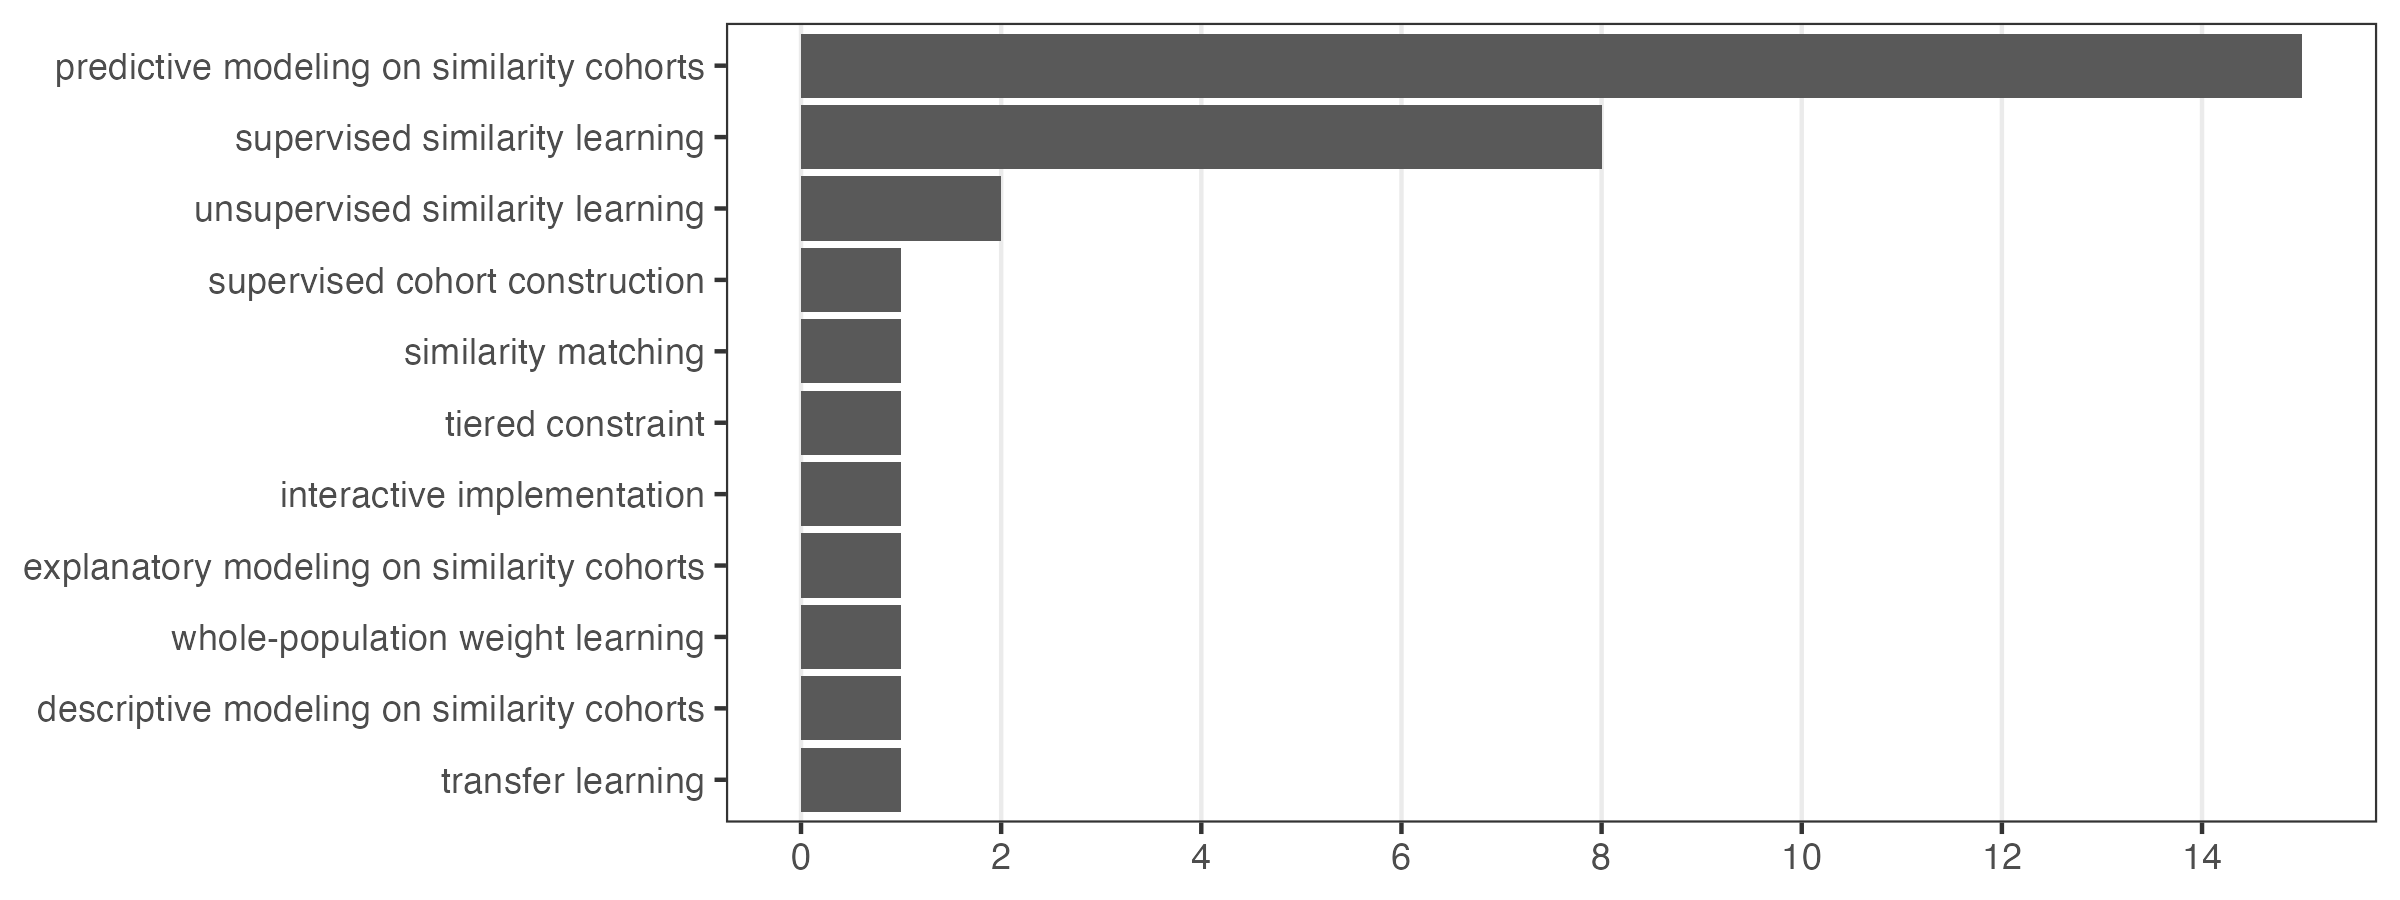
\includegraphics[width=1\linewidth]{Fig4} 

}

\caption{Frequency of recurring methodological elements across included studies.}\label{fig:methods}
\end{figure}

\subsection{\texorpdfstring{Rationales\hl{ for proposed methods}}{Rationales}}\label{rationales}

\hl{Our review was driven by an interest in the potential of SCBM toward interpretable ML. While not essential to the main text, we were therefore interested in understanding what needs motivated the various proposed methods we found.}

The included studies hypothesized, asserted, or assumed several benefits
of \hl{SCBM} specific to clinical and medical settings and advantages
over other modeling approaches. The most common was that the restriction
to similar or relevant past cases would improve predictive performance
for the index case \citep{Mariuzzi1997, Liang2015, Ng2015, Lee2017}. In
particular, \citet{Lee2015} hypothesized and confirmed that the value of
each past case would be positively related to its similarity to the
index case, an assumption built in to the weighting schemes of other
approaches. \citet{Lowsky2013} made a different case, that the fewer
parametric assumptions and complications of a CBR-style model would
allow for greater accuracy. Additionally, several investigators asserted
that the use of localized cohorts befit the clinical focus on the
individual patient rather than the population, without reference to
performance \citep{Song2006, Xu2008}.

In an interesting contrast, \citet{Tang2021} and \citet{Ng2021} argued
that their localized approach using the larger and more heterogeneous
populations covered by EHR-derived data could better capture the messy
and diverse lessons of everyday practice, as a counterpart to guidelines
based on randomized controlled trials. Their emphasis on the enabling
role of EHRs to power methods well-suited to large, structured data
repositories was shared by several others
\citep{CampilloGimenez2013, Nicolas2014, Verma2015, Lee2017}.
\citet{Verma2015} and \citet{Zhang2018} additionally pointed out that
\hl{SCBM}s are adaptable to noise in the data, variation in patterns of
missingness, and (harkening to the last step of the R4 cycle) addition
of new cases with known outcomes to the corpus. These properties, they
said, tend to be more difficult for whole-population models to handle.

The other frequent advantage attributed to \hl{SCBM} was
interpretability. \citet{Elter2007} and \citet{Nicolas2014} emphasized
the value of the detailed past cases, available to the user, on which
predictions are based. This ``self-explanation capability'' made outputs
more intelligible to physicians in the \hl{CDSS} setting. \citet{Ng2015}
additionally pointed out that localized GLMs yield localized effect
estimates, which may help investigators identify individually relevant
risk factors. \citet{Liu2022} took this idea further, systematically
comparing regression coefficients for specific risk factors across
dozens of diagnostic subpopulations. \citet{Doborjeh2022} used localized
time series models to identify environmental changes associated with
increased stroke risk.

The remaining coded rationales were for augmentations or hybridizations
of then-conventional CBR, most of which defended the use of other tools
to improve performance via cohort selection
\citep{CampilloGimenez2013, Nicolas2014, Vilhena2016} or to make models
and outputs more interpretable \citep{Lopez2011, Wang2019}.
\citet{Liang2015} argued for simultaneous optimization of cohort and
feature selection with model parameterization; their TWNFI approach
combines localization with regularization.

\subsection*{Performance evaluations and
comparisons}\label{performance-evaluations-and-comparisons}
\addcontentsline{toc}{subsection}{Performance evaluations and
comparisons}

Table \ref{tab:performance} summarizes the evaluations and comparisons
made of methods proposed in the included studies. In most cases, not all
performance results are included; for the sake of concision, only what
we judged to be the headline results, using the primary evaluation
metrics, are reproduced here. The table contains no original results.
\hl{Figure }\ref{fig:performance}\hl{ visualizes the relationship between the performances of the proposed methods (not of their comparators) and several aspects of the experiments used to evaluate them.}

\begin{landscape}

\textbf{TODO: Place vertical separators between major columns.}

\small

\begin{longtable}[]{@{}
  >{\raggedright\arraybackslash}p{(\columnwidth - 12\tabcolsep) * \real{0.1088}}
  >{\raggedright\arraybackslash}p{(\columnwidth - 12\tabcolsep) * \real{0.0725}}
  >{\raggedright\arraybackslash}p{(\columnwidth - 12\tabcolsep) * \real{0.1658}}
  >{\raggedright\arraybackslash}p{(\columnwidth - 12\tabcolsep) * \real{0.2435}}
  >{\raggedleft\arraybackslash}p{(\columnwidth - 12\tabcolsep) * \real{0.0984}}
  >{\raggedright\arraybackslash}p{(\columnwidth - 12\tabcolsep) * \real{0.2124}}
  >{\raggedleft\arraybackslash}p{(\columnwidth - 12\tabcolsep) * \real{0.0984}}@{}}
\caption{\label{tab:performance}Evaluations of proposed methods and
comparisons to alternative methods. (See original studies for full names
and descriptions.)}\tabularnewline
\toprule\noalign{}
\begin{minipage}[b]{\linewidth}\raggedright
Citation
\end{minipage} & \begin{minipage}[b]{\linewidth}\raggedright
Measure
\end{minipage} & \begin{minipage}[b]{\linewidth}\raggedright
Problem
\end{minipage} & \begin{minipage}[b]{\linewidth}\raggedright
Proposals
\end{minipage} & \begin{minipage}[b]{\linewidth}\raggedleft
\end{minipage} & \begin{minipage}[b]{\linewidth}\raggedright
Comparators
\end{minipage} & \begin{minipage}[b]{\linewidth}\raggedleft
\end{minipage} \\
\midrule\noalign{}
\endfirsthead
\toprule\noalign{}
\begin{minipage}[b]{\linewidth}\raggedright
Citation
\end{minipage} & \begin{minipage}[b]{\linewidth}\raggedright
Measure
\end{minipage} & \begin{minipage}[b]{\linewidth}\raggedright
Problem
\end{minipage} & \begin{minipage}[b]{\linewidth}\raggedright
Proposals
\end{minipage} & \begin{minipage}[b]{\linewidth}\raggedleft
\end{minipage} & \begin{minipage}[b]{\linewidth}\raggedright
Comparators
\end{minipage} & \begin{minipage}[b]{\linewidth}\raggedleft
\end{minipage} \\
\midrule\noalign{}
\endhead
\bottomrule\noalign{}
\endlastfoot
\citet{Wyns2004} & Accuracy & Arthritis & Kohonen + CBR &
75.60\%\hspace{6em} & Kohonen mapping & 54.70\%\hspace{6em} \\
& & & & \hspace{6em} & CBR & 60.40\%\hspace{6em} \\
& & & & \hspace{6em} & Quest & 50.90\%\hspace{6em} \\
& & & & \hspace{6em} & backpropagation & 54.70\%\hspace{6em} \\
\citet{Park2006} & Accuracy & Dermatology & Statistical CBR &
96.57\%\hspace{6em} & CBR & 95.43\%\hspace{6em} \\
& & & & \hspace{6em} & C5.0 & 93.71\%\hspace{6em} \\
& & & & \hspace{6em} & CART & 92.00\%\hspace{6em} \\
& & & & \hspace{6em} & LR & 91.14\%\hspace{6em} \\
& & & & \hspace{6em} & kNN & 88.29\%\hspace{6em} \\
& & Heart & Statistical CBR & 83.70\%\hspace{6em} & LR &
84.44\%\hspace{6em} \\
& & & & \hspace{6em} & kNN & 82.22\%\hspace{6em} \\
& & & & \hspace{6em} & CBR & 81.85\%\hspace{6em} \\
& & & & \hspace{6em} & CART & 76.67\%\hspace{6em} \\
& & & & \hspace{6em} & C5.0 & 76.30\%\hspace{6em} \\
& & Breast & Statistical CBR & 96.96\%\hspace{6em} & kNN &
97.50\%\hspace{6em} \\
& & & & \hspace{6em} & CBR & 96.61\%\hspace{6em} \\
& & & & \hspace{6em} & LR & 96.61\%\hspace{6em} \\
& & & & \hspace{6em} & C5.0 & 94.29\%\hspace{6em} \\
& & & & \hspace{6em} & CART & 92.14\%\hspace{6em} \\
& & Diabetes & Statistical CBR & 76.32\%\hspace{6em} & LR &
77.11\%\hspace{6em} \\
& & & & \hspace{6em} & CBR & 73.16\%\hspace{6em} \\
& & & & \hspace{6em} & C5.0 & 73.15\%\hspace{6em} \\
& & & & \hspace{6em} & CART & 72.89\%\hspace{6em} \\
& & & & \hspace{6em} & kNN & 65.39\%\hspace{6em} \\
& & Liver & Statistical CBR & 66.76\%\hspace{6em} & CART &
67.94\%\hspace{6em} \\
& & & & \hspace{6em} & LR & 67.35\%\hspace{6em} \\
& & & & \hspace{6em} & C5.0 & 66.47\%\hspace{6em} \\
& & & & \hspace{6em} & CBR & 60.88\%\hspace{6em} \\
& & & & \hspace{6em} & kNN & 55.59\%\hspace{6em} \\
\citet{Song2006} & RMSE & GFR & TWNFI & 7.08\hspace{6em} & MDRD &
7.74\hspace{6em} \\
& & & & \hspace{6em} & MLP & 8.38\hspace{6em} \\
& & & & \hspace{6em} & ANFIS & 7.40\hspace{6em} \\
& & & & \hspace{6em} & DENFIS & 7.22\hspace{6em} \\
& & & & \hspace{6em} & TNFI & 7.28\hspace{6em} \\
\citet{Elter2007} & AUROC & mammography mass region & CBR &
0.885\hspace{6em} & DT & 0.872\hspace{6em} \\
& & & & \hspace{6em} & ANN & 0.882\hspace{6em} \\
\citet{Xu2008} & Accuracy & Return-to-work & CBR & 62.5\%\hspace{6em} &
LR & 71.2\%\hspace{6em} \\
\citet{Kasabov2010} & Accuracy & Colon cancer diagnosis & TWNFI &
91.9\%\hspace{6em} & MLR (Personalized) & 82.3\%\hspace{6em} \\
& & & & \hspace{6em} & SVM (Personalized) & 90.3\%\hspace{6em} \\
& & & & \hspace{6em} & WKNN & 90.3\%\hspace{6em} \\
\citet{Liang2015} & Accuracy & Colon cancer & knnGSA &
85.48\%\hspace{6em} & SVM & 82.14\%\hspace{6em} \\
& & & svmGSA & 87.10\%\hspace{6em} & ECF & 72.30\%\hspace{6em} \\
& & & & \hspace{6em} & KNN & 82.14\%\hspace{6em} \\
& & & & \hspace{6em} & WKNN & 82.14\%\hspace{6em} \\
& & Leukemia & knnGSA & 97.22\%\hspace{6em} & SVM &
95.83\%\hspace{6em} \\
& & & svmGSA & 97.22\%\hspace{6em} & ECF & 94.44\%\hspace{6em} \\
& & & & \hspace{6em} & KNN & 94.44\%\hspace{6em} \\
& & & & \hspace{6em} & WKNN & 94.44\%\hspace{6em} \\
& & Lymphoma & knnGSA & 94.81\%\hspace{6em} & SVM &
93.51\%\hspace{6em} \\
& & & svmGSA & 94.81\%\hspace{6em} & ECF & 92.21\%\hspace{6em} \\
& & & & \hspace{6em} & KNN & 93.51\%\hspace{6em} \\
& & & & \hspace{6em} & WKNN & 93.51\%\hspace{6em} \\
& & Lung cancer & knnGSA & 98.34\%\hspace{6em} & SVM &
95.31\%\hspace{6em} \\
& & & svmGSA & 98.90\%\hspace{6em} & ECF & 92.87\%\hspace{6em} \\
& & & & \hspace{6em} & KNN & 96.60\%\hspace{6em} \\
& & & & \hspace{6em} & WKNN & 95.50\%\hspace{6em} \\
\citet{Lowsky2013} & Relative IPEC & Graft survival & MKNN &
0.973\hspace{6em} & RSF & 0.957\hspace{6em} \\
\citet{CampilloGimenez2013} & AUROC & Waitlist registration, complete &
CBR + Wj & 89.8\%\hspace{6em} & LR & 92.0\%\hspace{6em} \\
& & & CBR + Wk & 90.7\%\hspace{6em} & Standalone CBR &
90.4\%\hspace{6em} \\
& & & CBR + Wj + Wk & 87.4\%\hspace{6em} & & \hspace{6em} \\
& & Waitlist registration, stepwise & CBR + Wj & 82.7\%\hspace{6em} & LR
& 92.1\%\hspace{6em} \\
& & & CBR + Wk & 86.2\%\hspace{6em} & Standalone CBR &
91.4\%\hspace{6em} \\
& & & CBR + Wj + Wk & 88.5\%\hspace{6em} & & \hspace{6em} \\
\citet{Nicolas2014} & Accuracy & Nevus & Collaborative + rules &
98\%\hspace{6em} & Dermoscopy CBR & 92\%\hspace{6em} \\
& & & Collaborative + rules + DML & 100\%\hspace{6em} & Confocal CBR &
96\%\hspace{6em} \\
& & & & \hspace{6em} & Collaborative & 95\%\hspace{6em} \\
\citet{Ng2015} & AUROC & Diabetes onset & Personalized LR
(LSML+FeatureFiltering) & 0.624\hspace{6em} & KNN & 0.617\hspace{6em} \\
& & & Personalized LR (LSML) & 0.619\hspace{6em} & Global LR &
0.611\hspace{6em} \\
& & & Personalized LR (Euclidean) & 0.614\hspace{6em} & &
\hspace{6em} \\
& & & Personalized LR (Random) & 0.602\hspace{6em} & & \hspace{6em} \\
\citet{Lee2015} & AUROC & 30-day mortality & Individualized LR &
0.830\hspace{6em} & Individualized DC & 0.797\hspace{6em} \\
& & & Individualized DT & 0.753\hspace{6em} & & \hspace{6em} \\
\citet{Lee2017} & AUROC & & Individualized LR & 0.824\hspace{6em} &
Individualized DC & 0.801\hspace{6em} \\
& & & Individualized DT & 0.779\hspace{6em} & & \hspace{6em} \\
& & & Individualized RF & 0.839\hspace{6em} & & \hspace{6em} \\
& & & Individualized CSRF & 0.832\hspace{6em} & & \hspace{6em} \\
\citet{Malykh2018} & Accuracy & J13/pneumonia & & \hspace{6em} &
Case-based ANN & 81.6\%\hspace{6em} \\
& & K80.1/gallbladder & & \hspace{6em} & Case-based ANN &
76.7\%\hspace{6em} \\
& & H25.1/age-related cataract & & \hspace{6em} & Case-based ANN &
94.9\%\hspace{6em} \\
& & H26.2/complicated cataract & & \hspace{6em} & Case-based ANN &
91.4\%\hspace{6em} \\
& & 167.4/encephalopathy & & \hspace{6em} & Case-based ANN &
72.4\%\hspace{6em} \\
& & 167.9/CBD & & \hspace{6em} & Case-based ANN & 75.4\%\hspace{6em} \\
& & N20.1/ureter & & \hspace{6em} & Case-based ANN &
58.7\%\hspace{6em} \\
\citet{Zhang2018} & AUROC & Cognitive impairment & Gaussian process
regression with custom kernel & 0.92\hspace{6em} & linear regression
without regularization & 0.81\hspace{6em} \\
& & & & \hspace{6em} & LASSO regression & 0.85\hspace{6em} \\
& & & & \hspace{6em} & ridge regression & 0.87\hspace{6em} \\
& & & & \hspace{6em} & RF & 0.90\hspace{6em} \\
& & & & \hspace{6em} & gradient boosting regression tree &
0.91\hspace{6em} \\
& & & & \hspace{6em} & XGBoost & 0.91\hspace{6em} \\
& & & & \hspace{6em} & kernel support vector regressor &
0.92\hspace{6em} \\
& & Parkinson's disease & Gaussian process regression with custom kernel
& 0.875\hspace{6em} & linear regression without regularization &
0.820\hspace{6em} \\
& & & & \hspace{6em} & ridge regression & 0.798\hspace{6em} \\
& & & & \hspace{6em} & RF & 0.734\hspace{6em} \\
& & & & \hspace{6em} & gradient boosting regression tree &
0.825\hspace{6em} \\
& & & & \hspace{6em} & kernel support vector regressor &
0.778\hspace{6em} \\
\citet{Wang2019} & AUROC & Diabetes & Personalized RF & 0.90\hspace{6em}
& & \hspace{6em} \\
& & & Personalized KNN & 0.82\hspace{6em} & & \hspace{6em} \\
& & & Personalized LR & 0.89\hspace{6em} & & \hspace{6em} \\
\citet{Ma2020} & AUROC & Discharge at 10 days & One-class JITL-ELM &
0.8510\hspace{6em} & ELM & 0.4973\hspace{6em} \\
& & & & \hspace{6em} & JITL-ELM & 0.2014\hspace{6em} \\
& & & & \hspace{6em} & One-class ELM & 0.7588\hspace{6em} \\
& & & & \hspace{6em} & One-class SVM & 0.4647\hspace{6em} \\
\citet{Liu2022} & AUROC & Acute kidney injury & & \hspace{6em} & Global
& 0.684\hspace{6em} \\
& & & & \hspace{6em} & Risk-ranking & 0.708\hspace{6em} \\
& & & & \hspace{6em} & PM-Kmeans & 0.721\hspace{6em} \\
& & & & \hspace{6em} & PM-Kmeans \& TL & 0.759\hspace{6em} \\
& & & & \hspace{6em} & PM-kNN & 0.732\hspace{6em} \\
& & & & \hspace{6em} & PM-kNN \& WS & 0.738\hspace{6em} \\
& & & & \hspace{6em} & PM-kNN \& TL & 0.769\hspace{6em} \\
& & & & \hspace{6em} & PM-kNN \& TL \& WS & 0.771\hspace{6em} \\
& & & & \hspace{6em} & PM-kNN \& WS \& SL & 0.744\hspace{6em} \\
& & & & \hspace{6em} & PMTL & 0.779\hspace{6em} \\
\citet{Doborjeh2022} & Accuracy & Stroke & Personalized SNN &
60.70\%\hspace{6em} & & \hspace{6em} \\
\end{longtable}

\normalsize

\end{landscape}

\begin{figure}[H]

{\centering 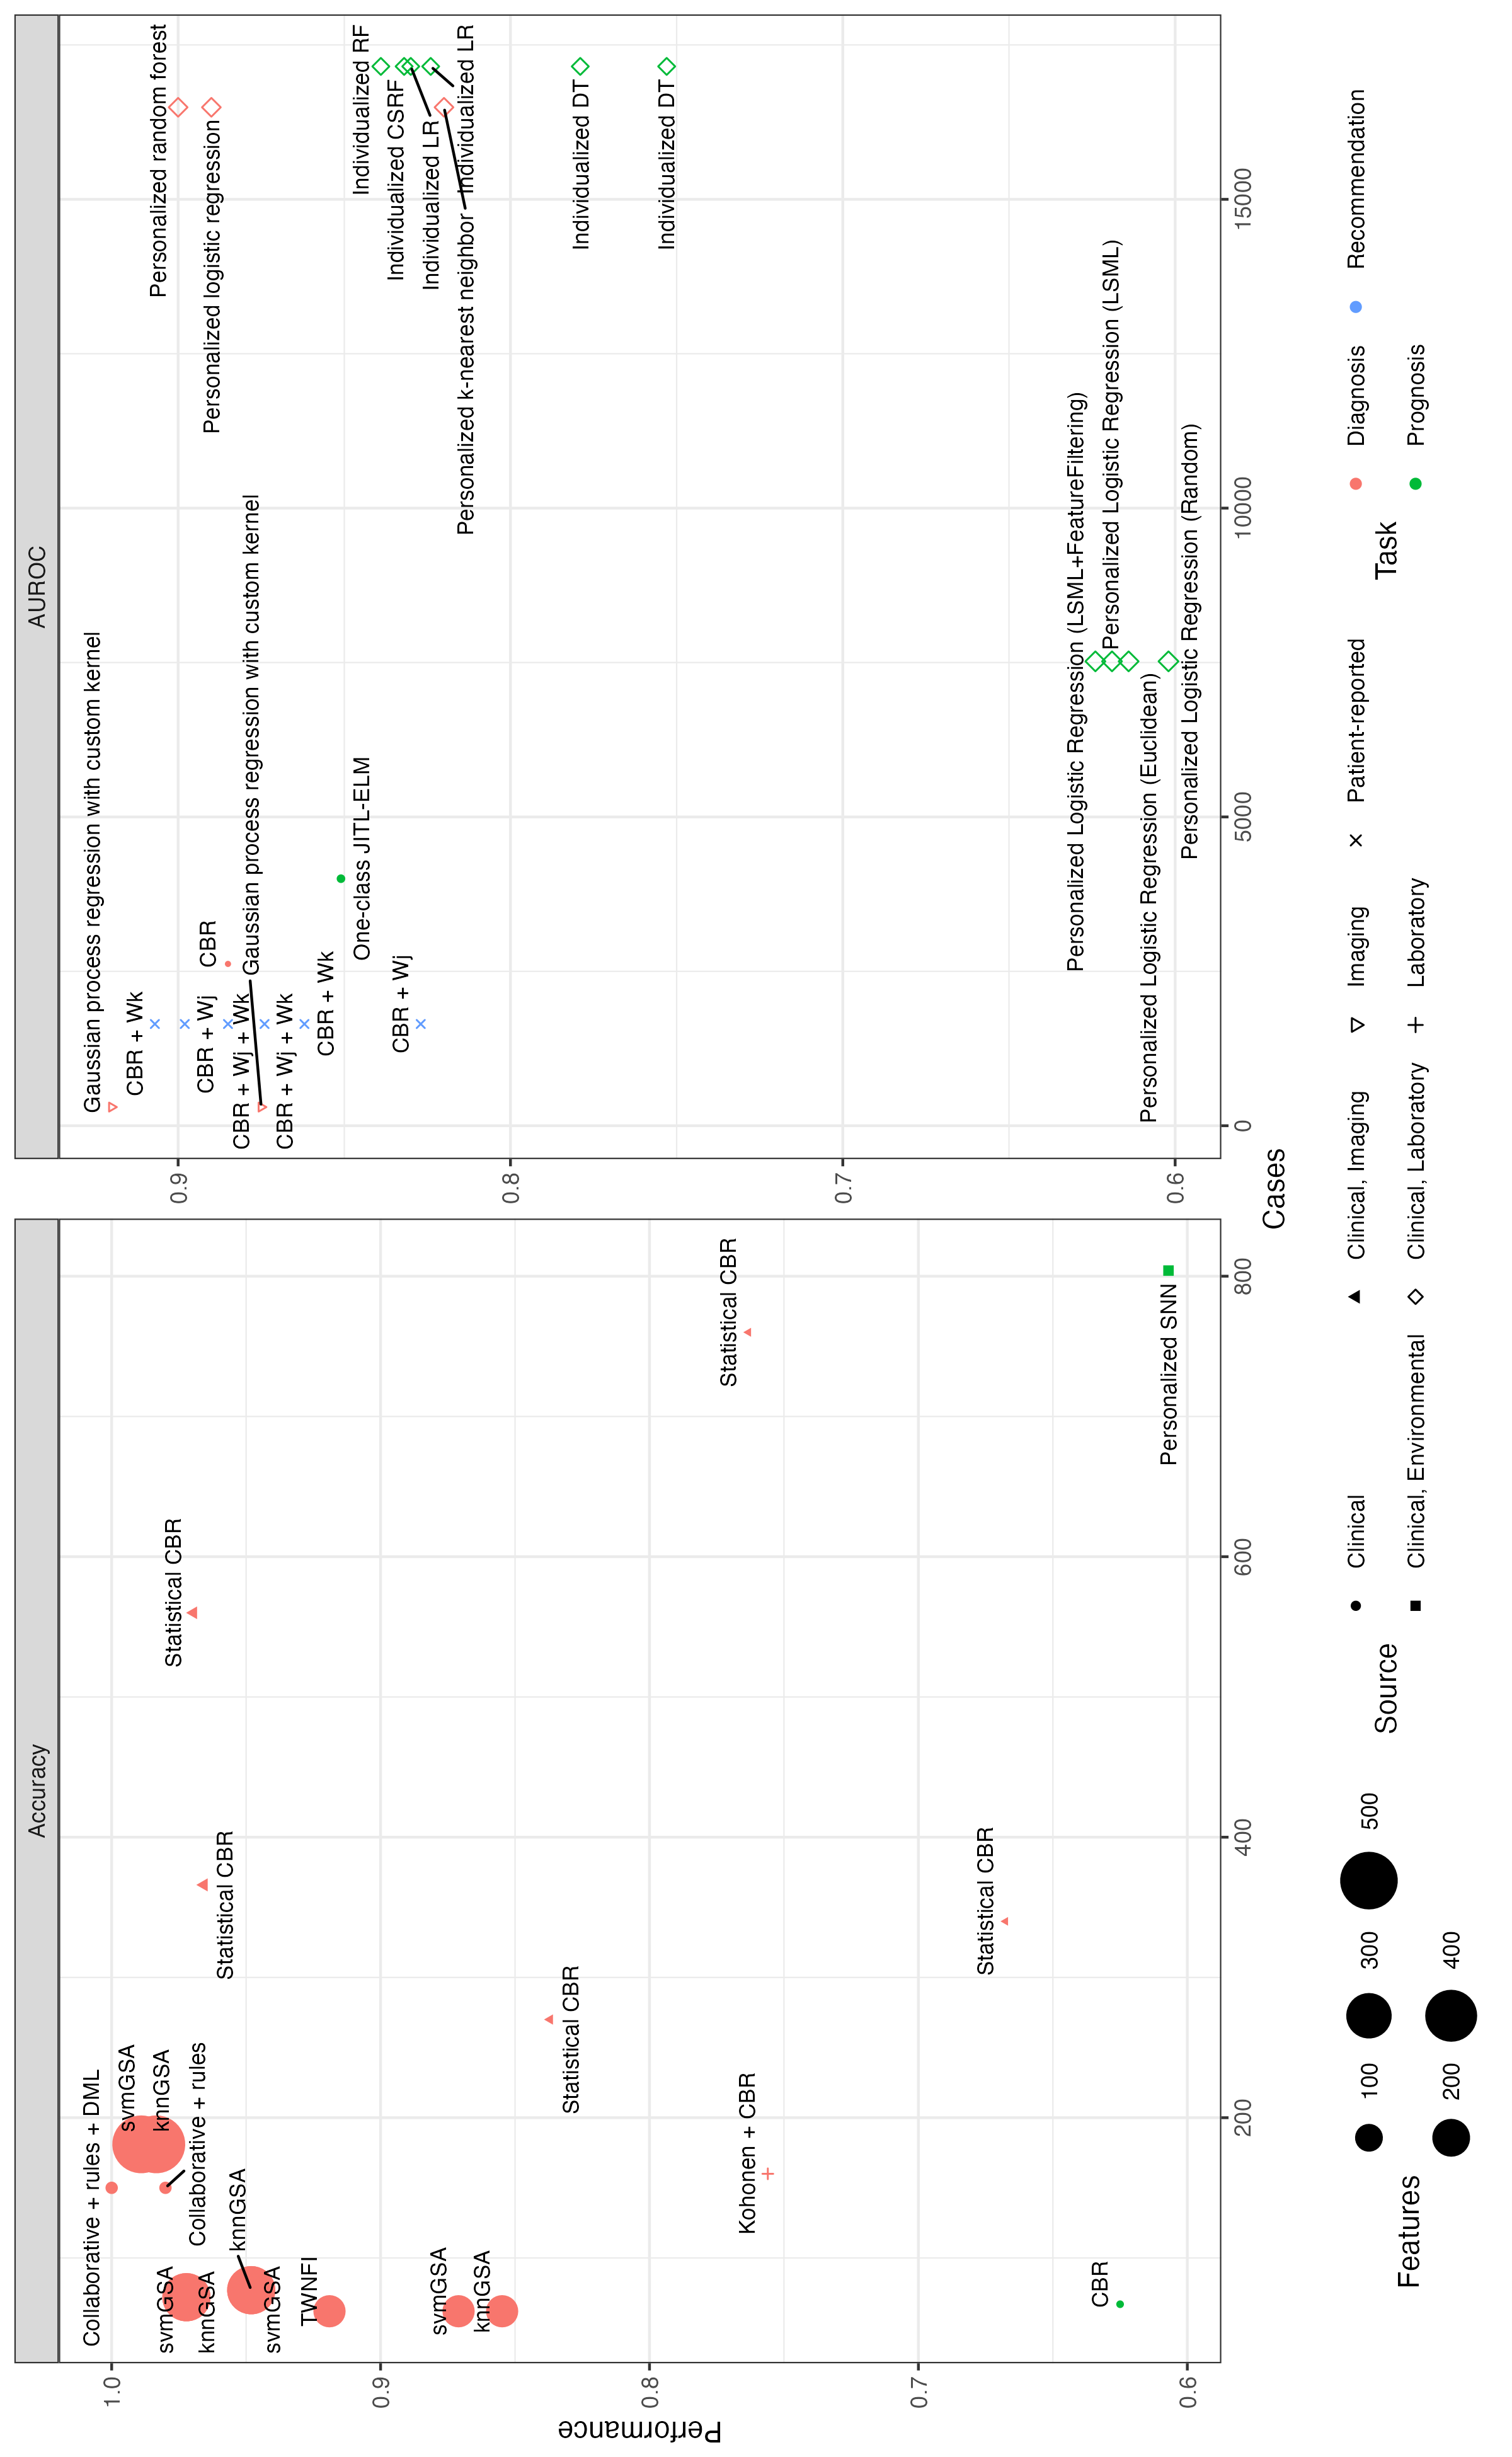
\includegraphics[width=1\linewidth]{Fig6} 

}

\caption{\hl{Scatterplot of predictive performance versus case count;
 marker size, shape, and color
 encode feature count, data source, and predictive task, respectively.
 (Image included as a separate file.)}}\label{fig:performance}
\end{figure}

\renewcommand\refname{References}
\bibliography{SR-bibliography.bib,SR-reviewers.bib,SR-0-Found.bib,SR-2-Included.bib,SR-3-Tracked.bib,SR-5-Screened.bib}


\end{document}
